\section{Introduction}
\label{sec:Introduction}

In phylogenetic reconstruction, evolution is generally seen as a stochastic process, whereby point mutations at the level of individuals are then subject to selection and genetic drift, leading to substitutions at the level of the population.
Under this framework, the past history of substitutions can be inferred from present-day populations, since each population have been shaped by a particular past-history evolutionary scenario.
As a result, present-day molecular \acrshort{DNA} sequences inform us theoretically on long-term trends in mutation, selection and genetic drift.
Independently, ecological properties such as phenotypic characters or life-history traits can be observed on extinct or present-day species, and reconstructed for the unobserved ancestral species.
Together, evolutionary and ecological mechanisms can be unravelled by comparing past history of ecological traits and their changes with regards to mutation, selection and genetic drift.

Practically, in order to disentangle mutation, selection and genetic drift shaping molecular sequences along the phylogenetic tree, we need to decompose our substitutions into different categories, where each category is subject to contrasted strength of mutation, selection and genetic drift.
In protein-coding \acrshort{DNA} sequences, the mutational process occurs at the \acrshort{DNA} level, whereas selection can be assumed to occur only at the protein level in first approximation.
Assuming synonymous substitutions are selectively neutral allows us to infer the pattern of mutation, without interference of selection.
Non-synonymous substitutions change the amino-acid sequence, and by comparing the substitution rates relative to the synonymous substitution rate (the ratio $\dnds$), we can estimate the global strength of selection exercised on a protein.
Such method has been leveraged in original codon models~\citep{Muse1994,Goldman1994} to detect proteins under adaptive selection.
However, the detection of adaptive evolution has been proved difficult since both pervasive purifying selection and adaptation are entangled into $\dnds$~\citep{Yang2000}.

In this context of pervasive purifying selection, the nearly-neutral theory predicts that changes in the global strength of selection (measured as $\dnds$) should be related to changes in genetic drift, mediated by effective population size ($\Ne$)~\citep{Ohta1992}.
Mechanistically, population with high $\Ne$ would more strongly purify deleterious mutations, resulting in lower $\dnds$~\citep{Kimura1979, Welch2008}.
As to observe these changes of purifying selection along the phylogeny, codon models estimate different $\dnds$ for different parts of the tree~\citep{Dutheil2012}, or with independent $\dnds$ for every branch of the tree~\citep{Popadin2007}.
Alternatively, $\dnds$ can be modelled as a continuous trait, varying along the phylogeny as a stochastic process, splitting at each node of the tree into independent processes~\citep{Seo2004,Lartillot2011}.
Once empirical changes $\dnds$ are estimated, they can be compared to changes in $\Ne$ across lineages such as to test the validity of the nearly-neutral theory prediction.

Independent estimation of $\Ne$ is usually done vie proxies, such as lineage with a low $\Ne$ typically correspond to population with large body size and extended longevity~\citep{Romiguier2014}, and polymorphic diversity at neutral markers is also a proxy of $\Ne$~\citep{Galtier2016}.
Using these proxies suggest a negative correlation between estimated $\dnds$ and $\Ne$~\citep{Popadin2007, Lanfear2010, Romiguier2014}, thus confirming the theoretical prediction.
Thereafter, integrative inference has been developed, jointly modelling the variation of life-history traits and $\dnds$ altogether, via a single multivariate Brownian process~\citep{Lartillot2011}.
Applications of this integrative approach also found that $\dnds$ correlates positively with traits such as longevity and body mass~\citep{Lartillot2011, Figuet2017}.
However, the universality and robustness of the correlation between $\dnds$ and life-history traits is still debated, and further investigations are required~\citep{Nabholz2013,Lanfear2014,Figuet2016, Bolivar2019}.
Moreover, the relationship between $\Ne$ and $\dnds$ is far for from being linear nor $1$-to-$1$, due to contrasted effect of selection merged into a single phenomenological parameter and due to non-equilibrium properties~\citep{Jones2016}.
Specifically, $\dnds$ is a function of $\Ne$ depending on the specific underlying modelling of selection, and the relationship can be approximated only if the selection coefficients are known to come from determined and fixed distribution~\citep{Nielsen2003, Welch2008}.
Hence, the predicted relationship between $\dnds$ and $\Ne$ is only obtained under specific a priori assumptions about the selective process.

Instead, mechanistic codon models explicitly introduced population-genetics equations into phylogenetic codon models~\citep{Halpern1998}.
These so-called mutation-selection codon models assign a different fitness for each amino acid, where the vector of 20 fitnesses is known as fitness profile, providing a model of purifying selection where the least fit amino acids are purified away.
Apart from selective effects between amino acids, the strength of selection is not typically homogeneous along the protein sequence, and depends on the local physicochemical requirements~\citep{Echave2016, Goldstein2016,Goldstein2017}.
In this context, local change in selective strength is usually taken into account by allowing site-specific amino-acid fitness profiles.
The sparsity of signal per codon site, however, requires to aggregate sites in categories, such as to gather enough signal for each amino-acid fitness profile.
Conversely, the category assigned to each site is chosen such that the sites aggregated into the same category share patterns of selection and hopefully the same physicochemical properties.
These methods developed to estimate site-heterogeneous amino-acid fitness profiles relied on penalized-likelihood~\citep{Tamuri2012,Tamuri2014}, or a Bayesian nonparametric random-effect approach~\citep{Rodrigue2010,Rodrigue2014,Rodrigue2016}.
Moreover, modelling explicitly purifying selection proved to be a valuable null (nearly-neutral) model~\citep{Spielman2015, DosReis2015}, against which to test for the presence of adaptation~\citep{Rodrigue2016,Bloom2017}.
However, these mutation-selection methods allowing site-specific patterns, have so far assumed the strength of genetic drift, or equivalently $\Ne$, to be constant across the phylogeny.

Relaxing the assumption of constant $\Ne$ in mutation-selection codon models is thus necessary to account for empirically grounded assumptions.
Moreover, the mutation-selection formalism incorporates explicitly $\Ne$ as a parameter of the model.
This formalism gives us leverage to revisit the correlations between ecological life-history traits (longevity, maturity, weight, size, \ldots) to effective population size~($\Ne$) and mutation rate per unit of time~($\mu$).
Altogether, can we mathematically model long-term fluctuation of $\Ne$ in mutation-selection codon model?
Empirically, do we have enough signal in alignment data, and computational tools, to estimate fluctuations of $\Ne$?


\section{New approaches}
\label{sec:NewApproaches}

Here we introduce a model of site-heterogeneous selection, and branch-heterogeneous traits~($\mu$, $\Ne$ and life-history traits), as depicted in figure~\ref{fig:modelSummary}.
Our model can be seen as the integration between the mutation-selection framework estimating site-heterogeneous selection coefficients~\citep{Rodrigue2014,Tamuri2014}, and the molecular comparative framework modelling the joint evolution of life-history and molecular traits~\citep{Lartillot2011}.
We test our model and inference framework against simulated data made under more realistic assumptions, and with empirical data while correlating life-history traits and population-genetics parameters of evolution.
Broadly, this framework aims to shade light on the long-term ecological and evolutionary process shaping the history of molecular sequences.

\begin{figure}[htbp]
    \centering
    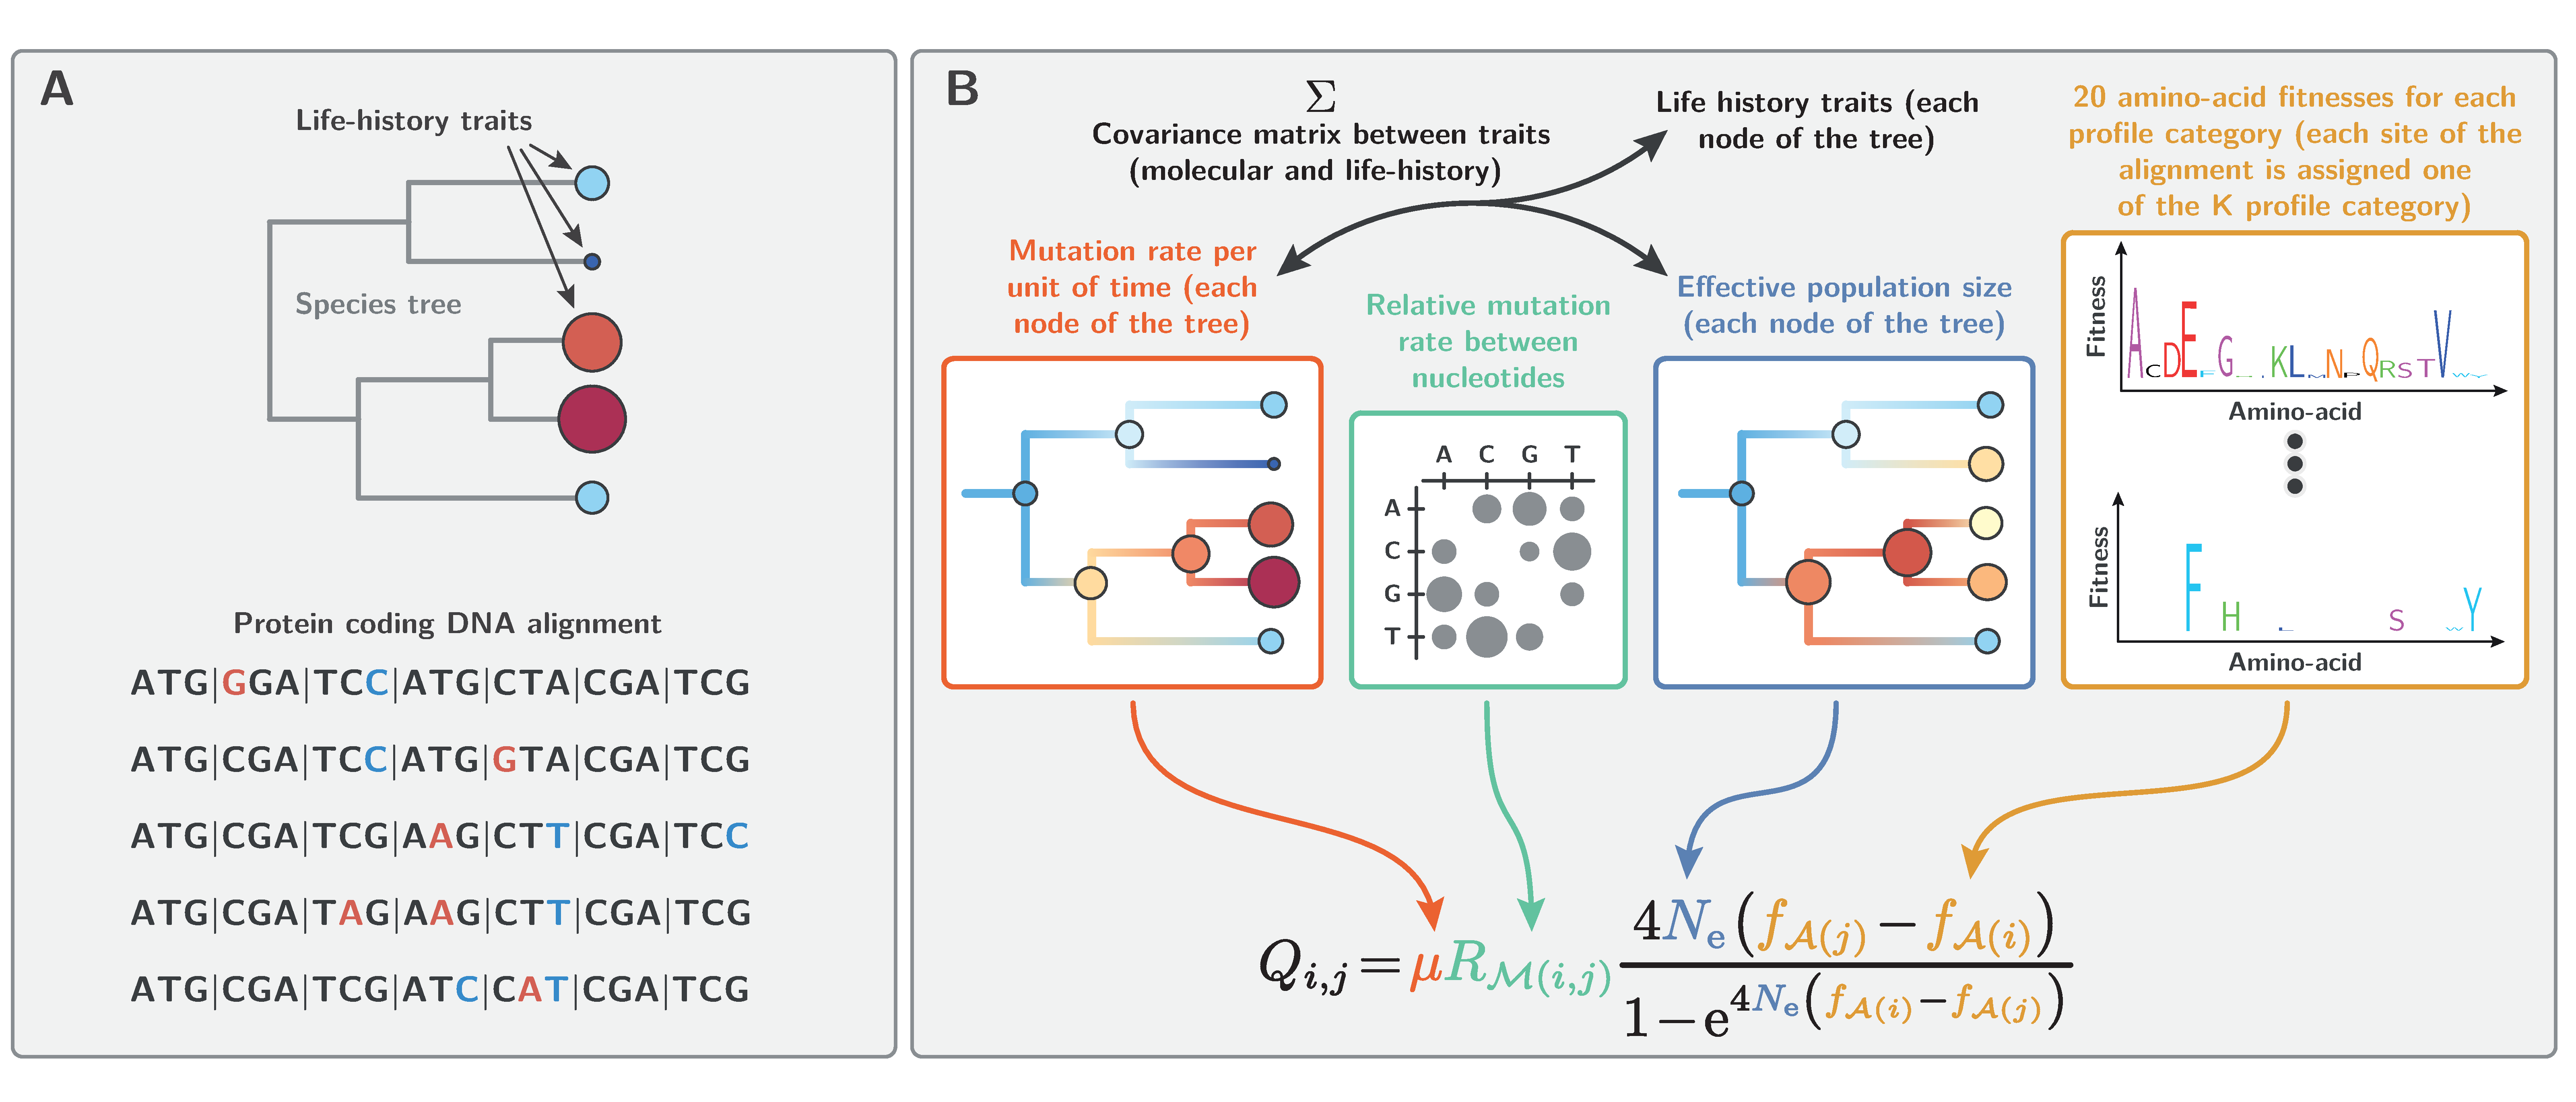
\includegraphics[width=\textwidth] {model_summary.pdf}
    \caption[Model summary]{
    Model summary.
    Panel A.
    Our method requires a given rooted topology, and an alignment of protein-coding \acrshort{DNA} for the extant species.
    Optionally, the method can use quantitative life-history traits at the leaves of the tree, and dated estimation for the internal nodes of the tree.
    Panel B.
    Our Bayesian inference model estimates selection coefficients, mutation rate, intensity of genetic drift and the age of the internal nodes.
    Effective population since~($\Ne$) and mutation rate per unit of time~($\mu$) are considered fluctuating branch-wise, but assumed constant across all sites of the \acrshort{DNA} sequence.
    Conversely, the selection coefficient of amino acids are considered changing for sites along the \acrshort{DNA} sequence, but are considered constant across the tree.
    Branch heterogeneity is modelled as an auto-correlated log-Brownian process, meaning our model estimates correlation coefficients between quantitative traits (as input), $\Ne$, and $\mu$, where phylogenetic inertia is accounted for.
    Synonymous substitutions are leveraged to estimates branch-wise mutation rate~($\mu$).
    Site-specific rates of non-synonymous substitutions across the tree is leveraged to estimate site-wise selection coefficient~($\Fit$).
    Branch-specific rates of non-synonymous substitutions across the sequence is leveraged to estimate branch-wise genetic drift~($\Ne$).
    }
    \label{fig:modelSummary}
\end{figure}

Formally, \acrshort{DNA} coding sequences are modelled at the level of the codon, where for each codon site (triplet of nucleotides), a change of codon means a change in \acrshort{DNA} but not necessarily in amino acid.
The substitution rate (per unit of time) from codon $\ci$ to $\cj$, denoted $\submatrix_{\itoj}$, is equal to the total rate of mutation (per unit of time) at the level of the population~($2\Ne\mu_{\itoj}$) multiplied by the probability of fixation of the mutation:
\begin{equation}
{\submatrix_{\itoj}}
    = 2 \Ne \mu_{\itoj} \pfix(\itoj)
\end{equation}
In the case of synonymous mutations, which we assumed are neutral, the probability of fixation is independent of the original and target codon, and equal $1/2 \Ne$.
Finally, ${\submatrix_{\itoj}}$ simplifies to:
\begin{equation}
    \submatrix_{\itoj} = \mu_{\itoj}
\end{equation}
The mutation rate $\mu_{\itoj}$ depends on the underlying nucleotide change between the codons $\ci$ and $\cj$.
First, if codon $\ci$ to $\cj$ are not neighbours, $\mu_{\itoj}$ is equal to $0$.
Second, if codon $\ci$ and $\cj$ are only one mutation away, $\mu_{\itoj}$ is given by the nucleotide relative rate~(${\mutmatrix_{\nucitoj}}$) scaled by the mutation rate per time~($\mu$).
Technically, the $4$-dimensional nucleotide relative rate matrix~($\Mutmatrix$) is normalized such that we expect $1$ substitution per unit of time, hence the scaling by $\mu$.

In the case of non-synonymous mutations, the probability of fixation depends on the difference in fitness~\citep{Ohta1992} between the amino acid encoded by the initial and final codons:
\begin{equation}
    \label{eq:mutationSelection}
    {\submatrix_{\itoj}} = \mu_{\itoj} \dfrac{4 \Ne \left({\fitj - \fiti}\right)}{{1 - \e^{4 \Ne \left({\fiti - \fitj}\right)} }}
\end{equation}
where $\Fit$ is a $20$-dimensional vector specifying the log-fitness for each amino acid, and $\aai$ is the amino acid encoded by codon $i$.
We see from this equation that, $\fit$ and $\Ne$ are confounded, such that increasing the effective population size while decreasing the fitnesses by the same factor leads to the same substitution rate.

In the model presented in this manuscript, $\Ne$ and $\mu$ are allowed to vary between species (across branches) as a multivariate log-Brownian process, but assumed constant along the \acrshort{DNA} sequence.
In a multivariate log-Brownian process, traits are modelled together as a vector-valued time-dependent random process, parameterized by a covariance matrix between traits~($\Covariancematrix$).
Altogether, values of the multivariate process at each node of the tree, a covariance matrix and divergence times are jointly estimated.
Once the traits are sampled at all nodes, traits along each branch is taken as the average between extremities of this branch.
Technically, the precision matrix (invert of covariance matrix) is distributed as an invert Wishart, meaning the prior matrix is diagonal, pushing the correlation coefficients between traits toward $0$.
The work presented here implemented the branch heterogeneity in a Bayesian context, as in \texttt{CoEvol}~\citep{Lartillot2011}.
Conversely, amino-acid fitness profiles $\Fit$ are assumed to vary across sites, but are considered constant along the tree.
The work presented here relies on the Bayesian nonparametric random-effect approach, developed to estimate site-heterogeneous amino-acid fitnesses as in \texttt{PhyloBayes}~\citep{Rodrigue2010}.
Our Bayesian implementation, written in \texttt{C++} in the software \texttt{\texttt{BayesCode}}, is publicly available at \url{https://github.com/ThibaultLatrille/bayescode}.

The phylogenetic codon model presented here makes several additional assumptions on the evolutionary processes generating the observed alignment.
First, the species tree topology is supposed to be known, and each gene should match the species tree, meaning genes are strict orthologs (no paralogs and no horizontal transfers).
Second, there is no epistasis (interaction between sites), such that any position of the sequence has its own independent evolutionary process and a substitution at one position does not affect the substitution process at other positions.
Third, from a population genetic perspective, we assumed sites of the protein to be unlinked, or equivalently the mutation rate is low enough such that there is no Hill-Robertson interference nor genetic hitchhiking.
Fourth, we assume \acrshort{DNA} sequences to be representative of the species, not taking into account the sampling effect tending to over-represent weakly deleterious mutations present at low frequencies.


\section{Results}
\label{sec:Results}

\begin{figure}[htbp]
    \centering
    \begin{minipage}{0.32\linewidth}
        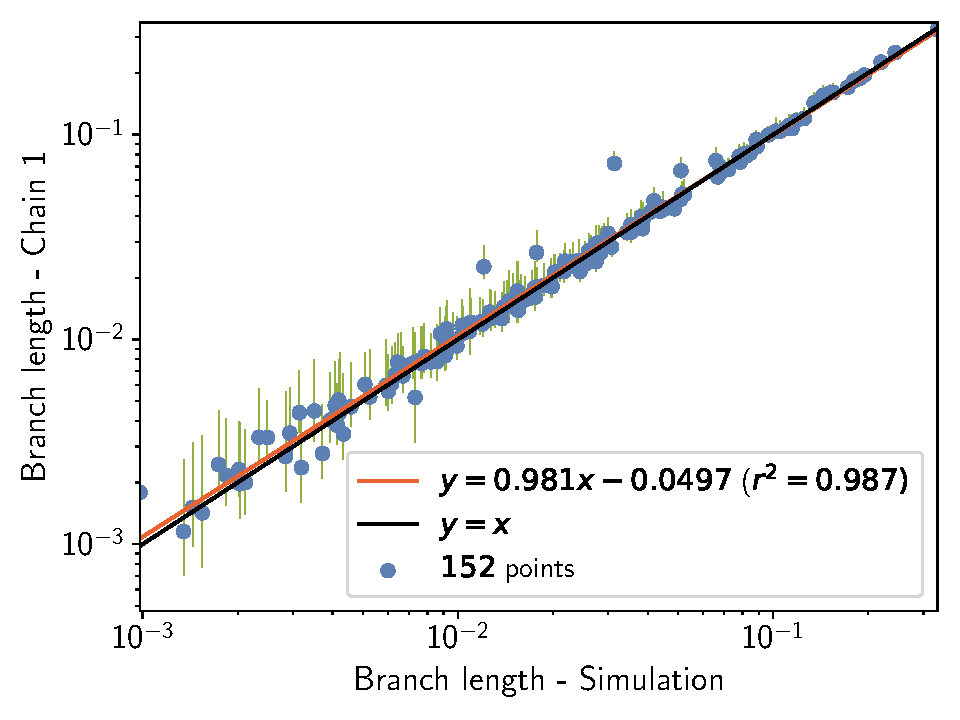
\includegraphics[width=\linewidth, page=1]{simulations/BranchWise_SimuDiv_SiteMutSelBranchNe_BranchCorrelation_Log10BranchLength}
    \end{minipage}
    \llap{\raisebox{-1.1cm}{\scriptsize A\hspace{0.35cm}}}\hfill
    \begin{minipage}{0.32\linewidth}
        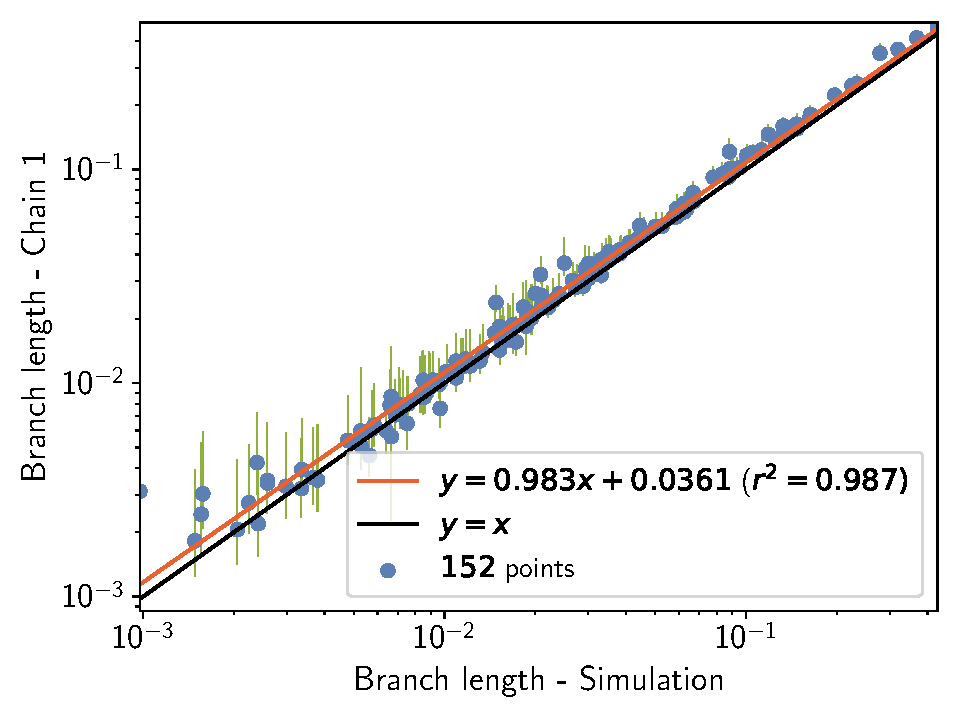
\includegraphics[width=\linewidth, page=1]{simulations/SimuPoly_SiteMutSelBranchNe_BranchCorrelation_Log10BranchLength}
    \end{minipage}
    \llap{\raisebox{-1.1cm}{\scriptsize B\hspace{0.35cm}}}\hfill
    \begin{minipage}{0.32\linewidth}
        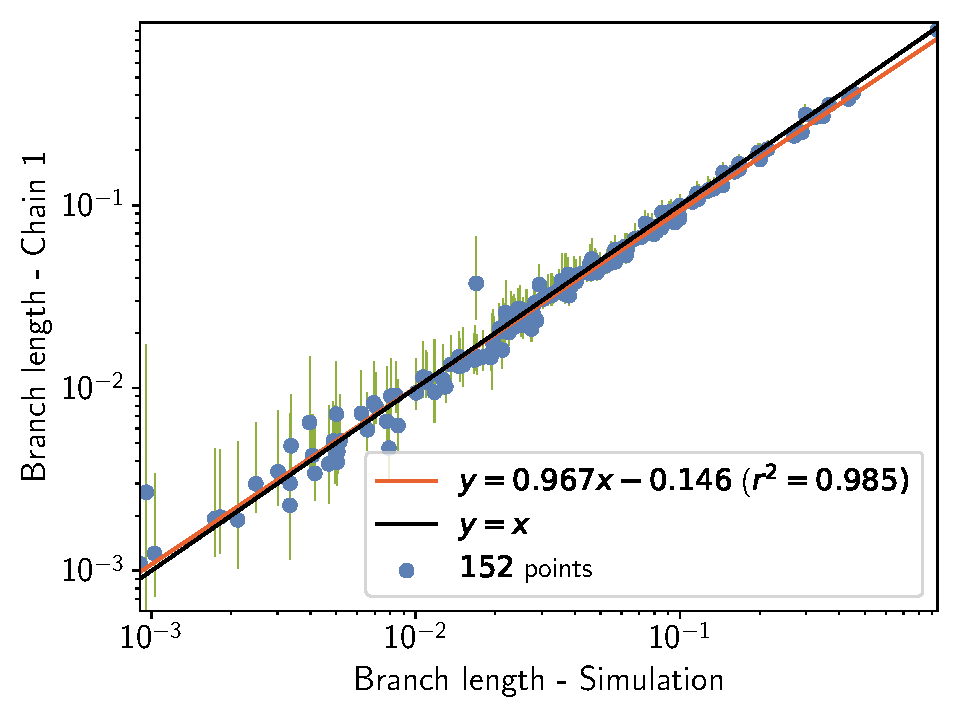
\includegraphics[width=\linewidth, page=1]{simulations/SimuFold_SiteMutSelBranchNe_BranchCorrelation_Log10BranchLength}
    \end{minipage}
    \llap{\raisebox{-1.1cm}{\scriptsize C\hspace{0.35cm}}}\hfill
    \begin{minipage}{0.32\linewidth}
        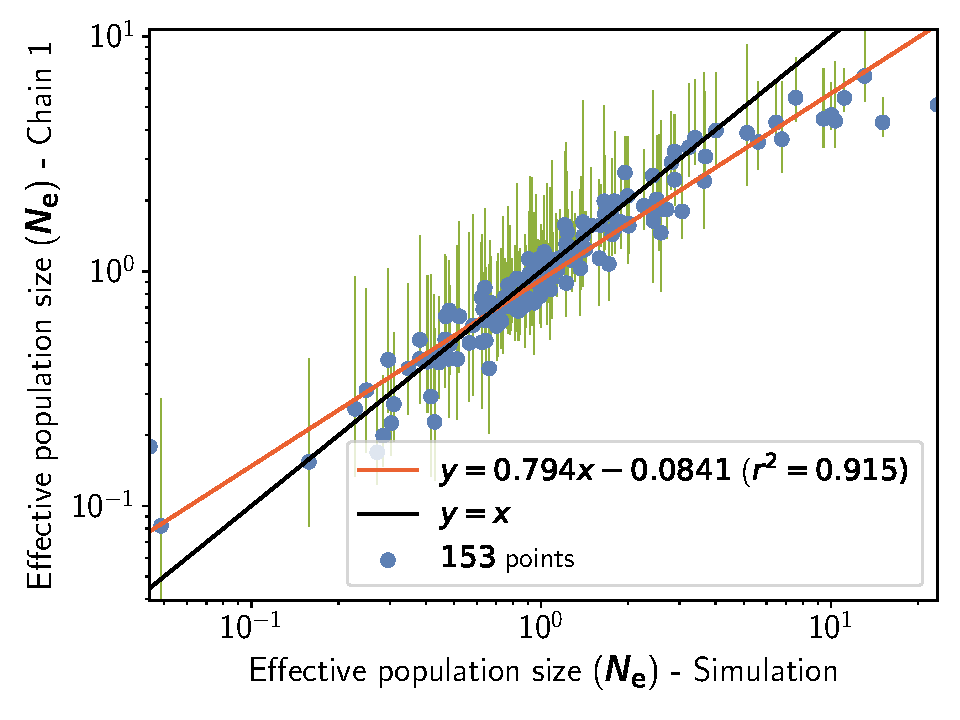
\includegraphics[width=\linewidth, page=1]{simulations/BranchWise_SimuDiv_SiteMutSelBranchNe_BranchCorrelation_LogPopulationSize}
    \end{minipage}
    \llap{\raisebox{-1.1cm}{\scriptsize D\hspace{0.35cm}}}\hfill
    \begin{minipage}{0.32\linewidth}
        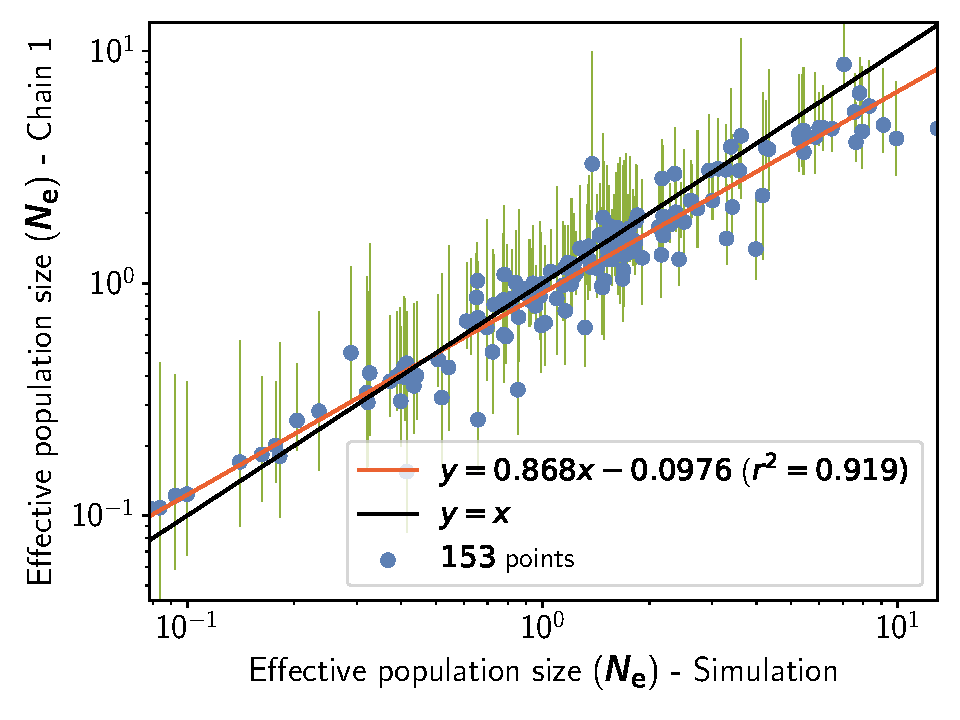
\includegraphics[width=\linewidth, page=1]{simulations/SimuPoly_SiteMutSelBranchNe_BranchCorrelation_LogPopulationSize}
    \end{minipage}
    \llap{\raisebox{-1.1cm}{\scriptsize E\hspace{0.35cm}}}\hfill
    \begin{minipage}{0.32\linewidth}
        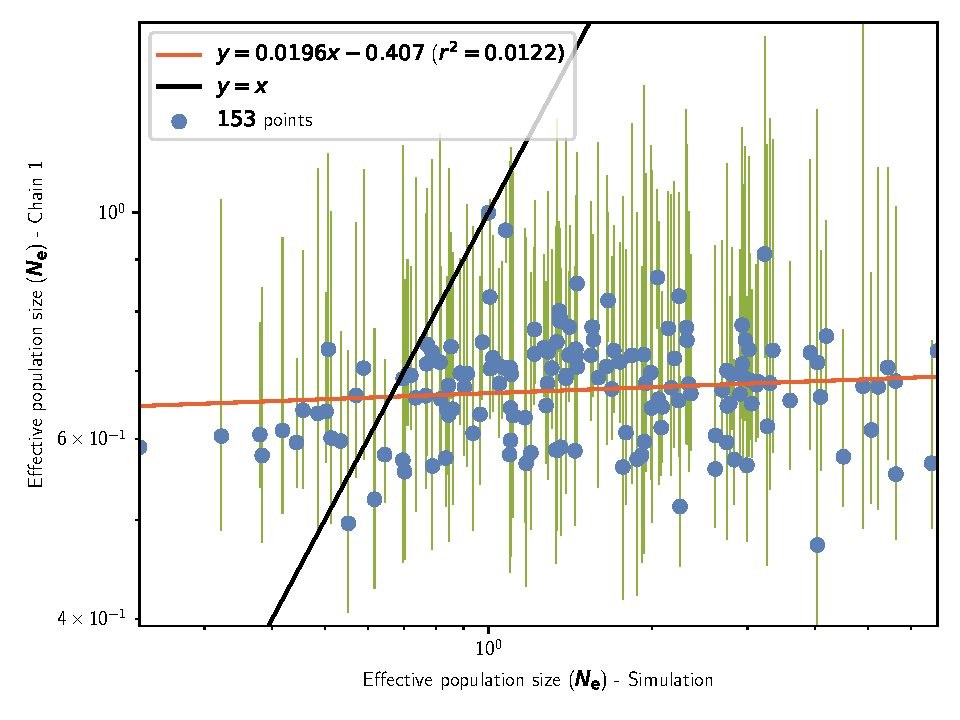
\includegraphics[width=\linewidth, page=1]{simulations/SimuFold_SiteMutSelBranchNe_BranchCorrelation_LogPopulationSize}
    \end{minipage}
    \llap{\raisebox{-1.1cm}{\scriptsize F\hspace{0.35cm}}}\hfill
    \caption[Inferred and simulated branch length and $\Ne$]{
    Inferred values in vertical axis against simulated value in horizontal axis.
    In the top row (panels A, B and C), branch length in expected number of substitutions for each branch of the tree.
    In the bottom row (panels D, E and F), $\Ne$ for each node (including leaves) of the tree, relative to $\Ne$ at the root of the tree.
    In the left panels (A and D), simulation under the mutation-selection approximation, as to test the soundness of the inference framework.
    In middle panels (B and E), simulation accounting for small population size effects~($5000$ individuals at the root), site linkage and short term fluctuation of $\Ne$.
    In the right panels (C and F), simulation accounting for site epistasis in context of selection for protein stability, with fluctuation of the selection coefficient along the phylogeny.
    The tree root is $150$ million years old, where the initial population start with a mutation rate of $\smash{1e^{-8}}$ per site per generation, and generation time of $10$ years.
    These experiments confirm that signal in the placental mammalian tree can allow to reliably infer the direction of change in $\Ne$, even if linkage disequilibrium, short term fluctuation of $\Ne$ and finite population size effects are not accounted for in the inference framework.
    However, the presence of epistasis between sites is a serious threat to the inference of $\Ne$.
    }
    \label{fig:simulations}
\end{figure}

\subsection{Simulated experiments}
\label{sec:ResultsSimulated}
The inference framework was first tested using independently simulated alignments (see Methods).
With the aim of applying the inference method to empirical dataset in placental mammals, the simulation parameters were chosen to match the empirical regime of total branch length (expected number of substitutions) from root to leaves.

A first series of simulations was meant to test the soundness of our inference framework, by simulating essentially under the model used for inference, although with an independently developed software.
The mutation-selection approximation was assumed to be valid, and sites were simulated under different fitness profiles.
In addition, $\Ne$ varies at the tree nodes but otherwise remains constant along each branch.
In this context, simulated branch length and $\Ne$ could be recovered appropriately by our inference method, as depicted in figure~\ref{fig:simulations}, panel A \& D.
Unfortunately, assumptions made for this simulations are almost certainly violated in practice.
First, $\Ne$ should change continuously along a branch, between each generation of the population.
Second, having a separate process for each site is equivalent to have no linkage between sites (free recombination), an assumption that should be relaxed.
Third, the probability of fixation (equation~\ref{eq:mutationSelection}) does not hold in small finite population.

For these reasons, we performed a second more challenging series of simulations.
The finite population was modelled explicitly in a Wright-Fisher simulator, tracking the frequency of each allele at each generation along the phylogeny.
Such simulator accounts for small population size effects, hitchhiking of weakly deleterious mutations during selective sweep and background selection due to linkage disequilibrium.
Fluctuations of $\Ne$ and mutation rate were also fluctuating continuously along the branch of the tree.
Moreover, noise was added by accounting for short-term fluctuations of $\Ne$ on the order of $20\%$ per generation.
The simulated branch length and $\Ne$ could be robustly recovered by the inference framework in this context, as depicted in figure~\ref{fig:simulations}, panel B \& E.

However, if the results are encouraging to apply the method on empirical data, we rely on the assumption of site-specific fitness landscape, which is almost certainly broken in practice.
Finally, we implemented a more complex, site-dependent fitness landscape accounting for the $3$-dimensional structure of protein and interaction between sites.
In such a model, the conformational stability of the protein determines the probability of being in the folded state, a proxy for fitness~\citep{Williams2006, Goldstein2011, Pollock2012}.
During a simulation, at a particular codon site, the fitness landscape is dependent on the actual amino acids present in the vicinity of this particular site (see section~\ref{subsec:protein-folding-probability} in supplementary materials).
Our inference framework could recover the simulated branch length (figure~\ref{fig:simulations}, panel C), but hardly retrieves the simulated $\Ne$ in the context of site-dependent epistasis (figure~\ref{fig:simulations}, panel F).
This effect can, however, be explained by the predicted independence of $\dnds$ to changes in $\Ne$ in this specific model of protein stability~\citep{Goldstein2013}.
Such independence between $\dnds$ and $\Ne$ is due to the structure of the fitness landscape, where a decrease in $\Ne$ leads to a sequence further to the optimal protein where the curvature of the fitness landscape is steeper, resulting in a higher selection coefficient exactly compensating the decrease in $\Ne$, and the scaled selection coefficient is (almost) constant.
Additionally, under a Fisher geometric landscape developed in supplementary materials (section~\ref{subsec:fisher-geometric-landscape}) and also incorporating epistasis, branch length is reliably estimated while $\Ne$ is also more difficult to estimate.

\subsection{Empirical experiments}
\label{sec:ResultsEmpirical}
\begin{figure}[htbp]
    \centering
    \begin{minipage}{0.411\linewidth}
        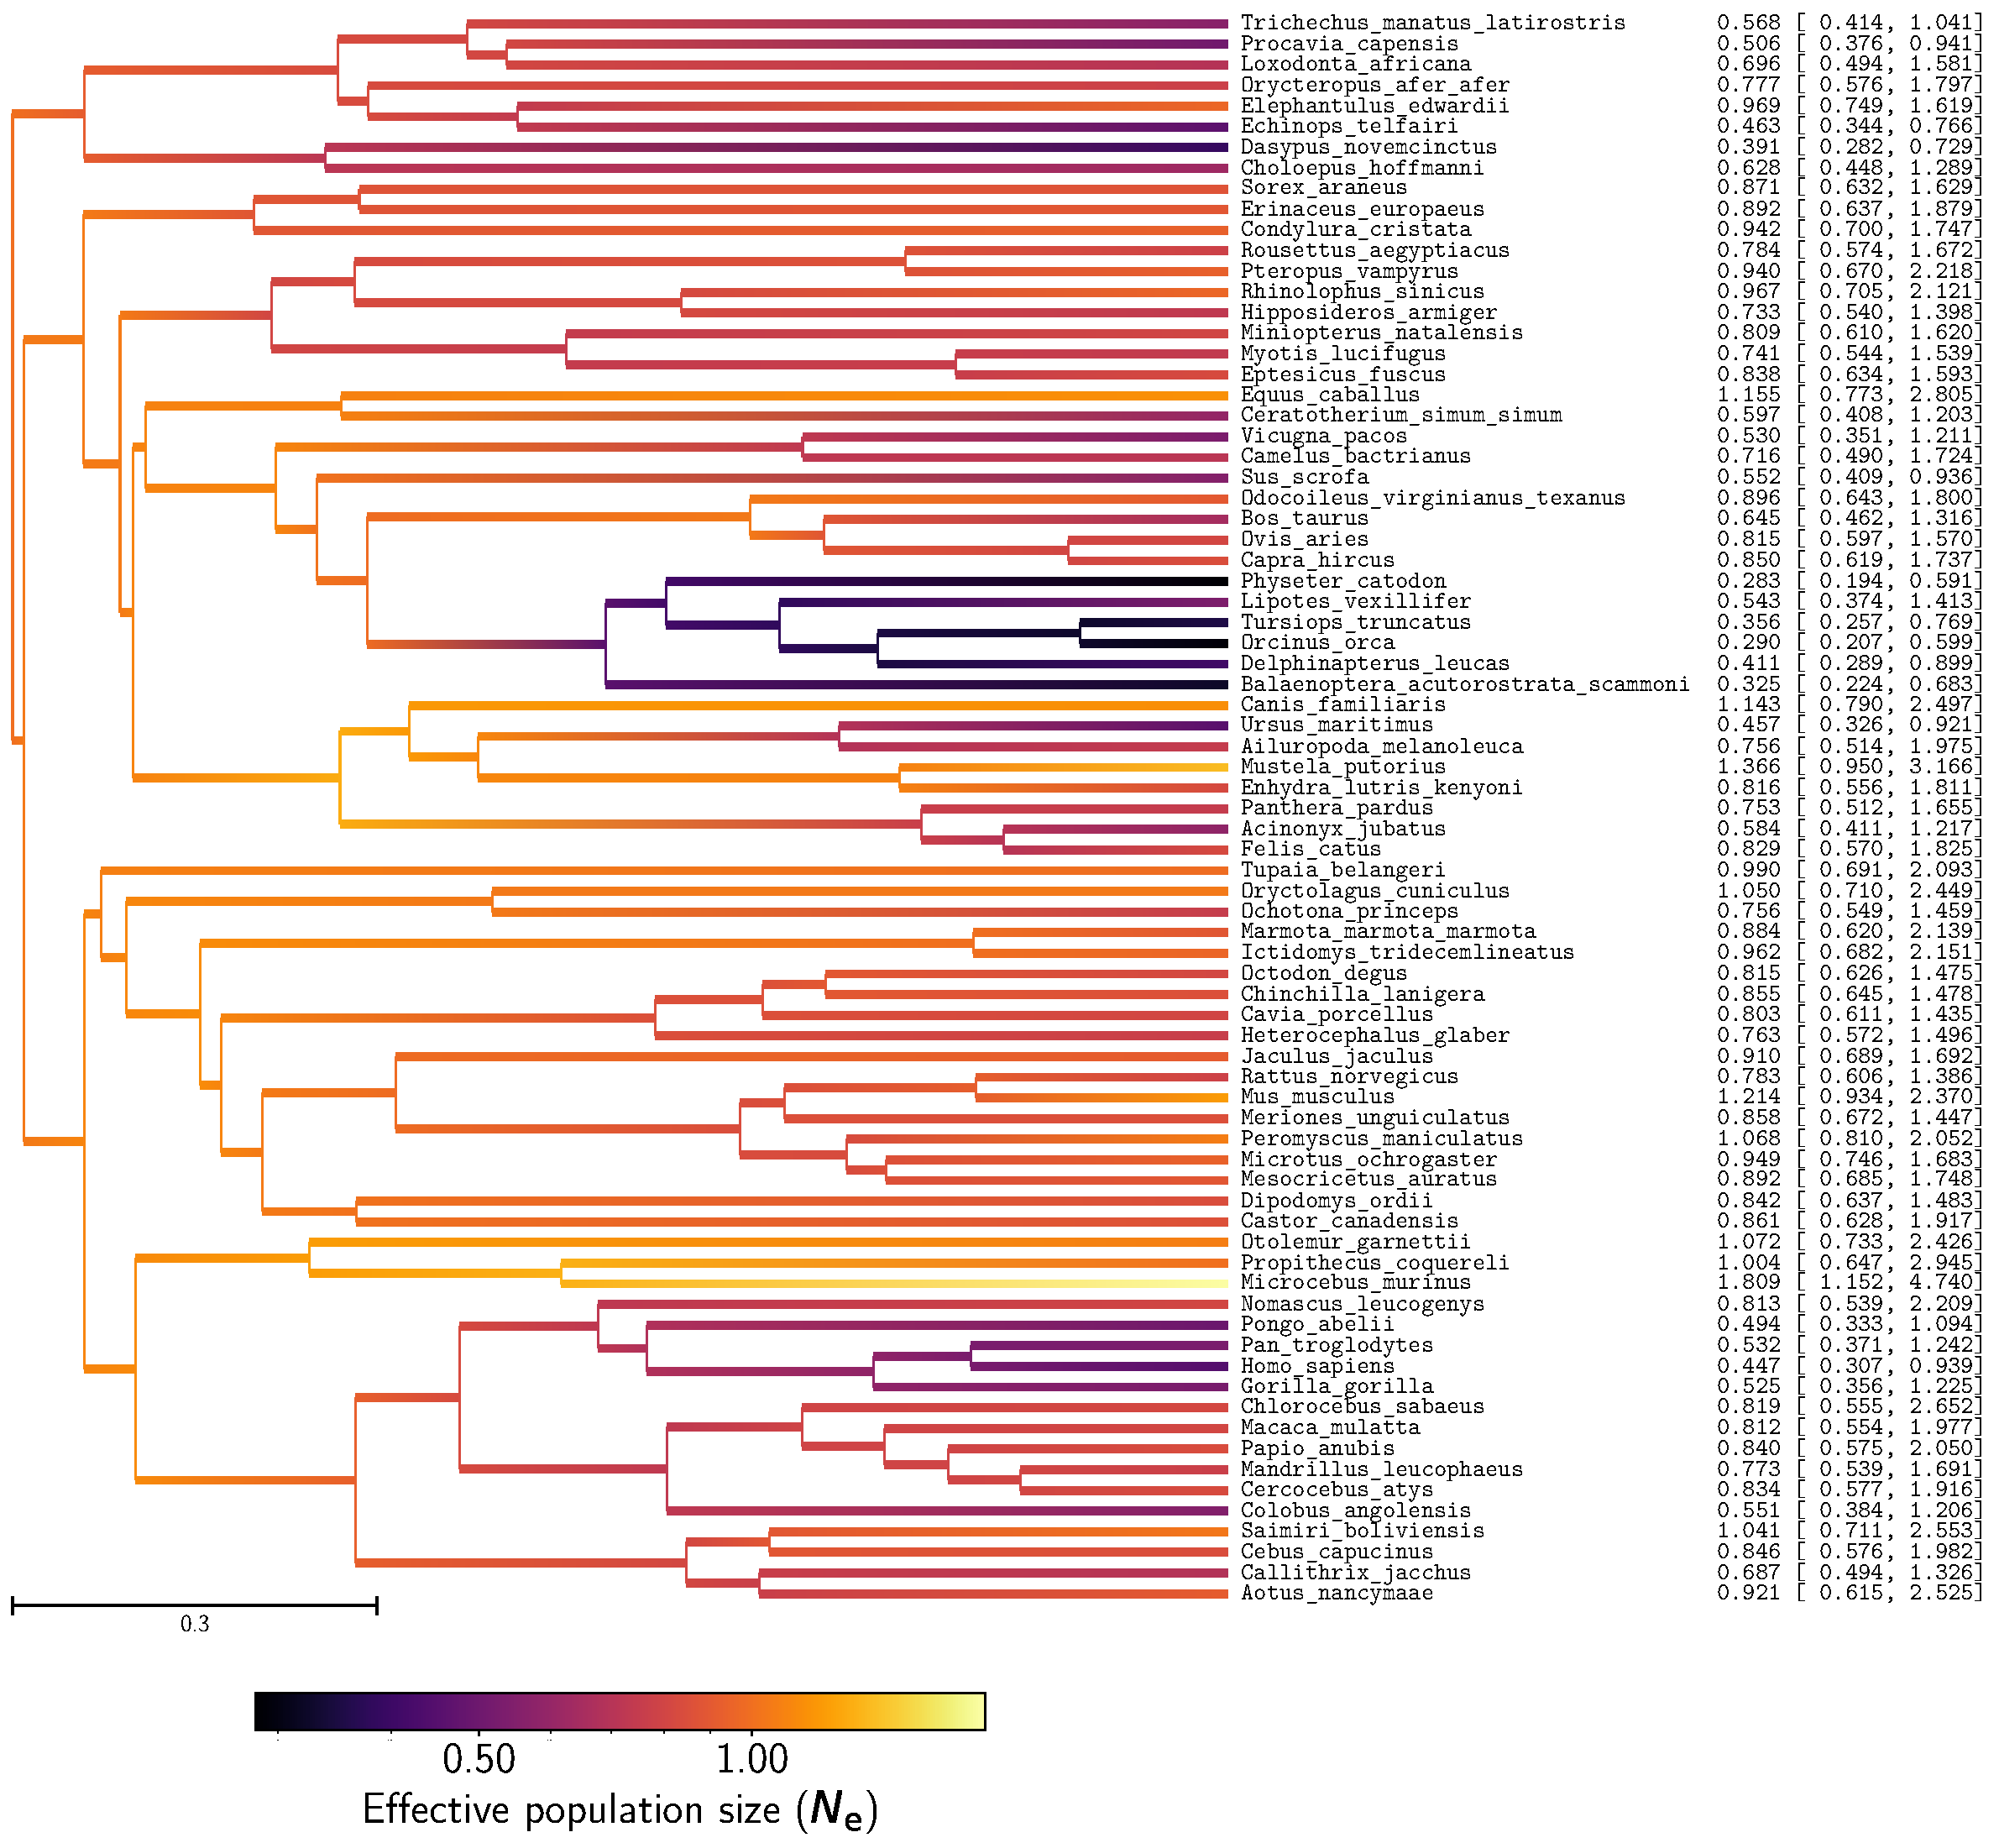
\includegraphics[valign=t, width=\linewidth, page=1, clip, trim=0cm 0cm 15.35cm 0.15cm]{mammals/18CDS_SiteMutSelBranchNe_R1_LogPopulationSize}
    \end{minipage}
    \begin{minipage}{0.158\linewidth}
        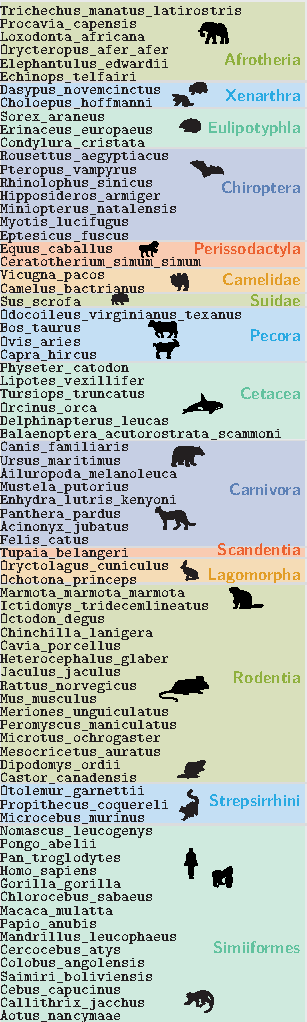
\includegraphics[valign=t, width=\linewidth, page=1, clip, trim=0cm -2.2cm 0cm 0cm]{mammals_species}
    \end{minipage}
    \begin{minipage}{0.411\linewidth}
        \reflectbox{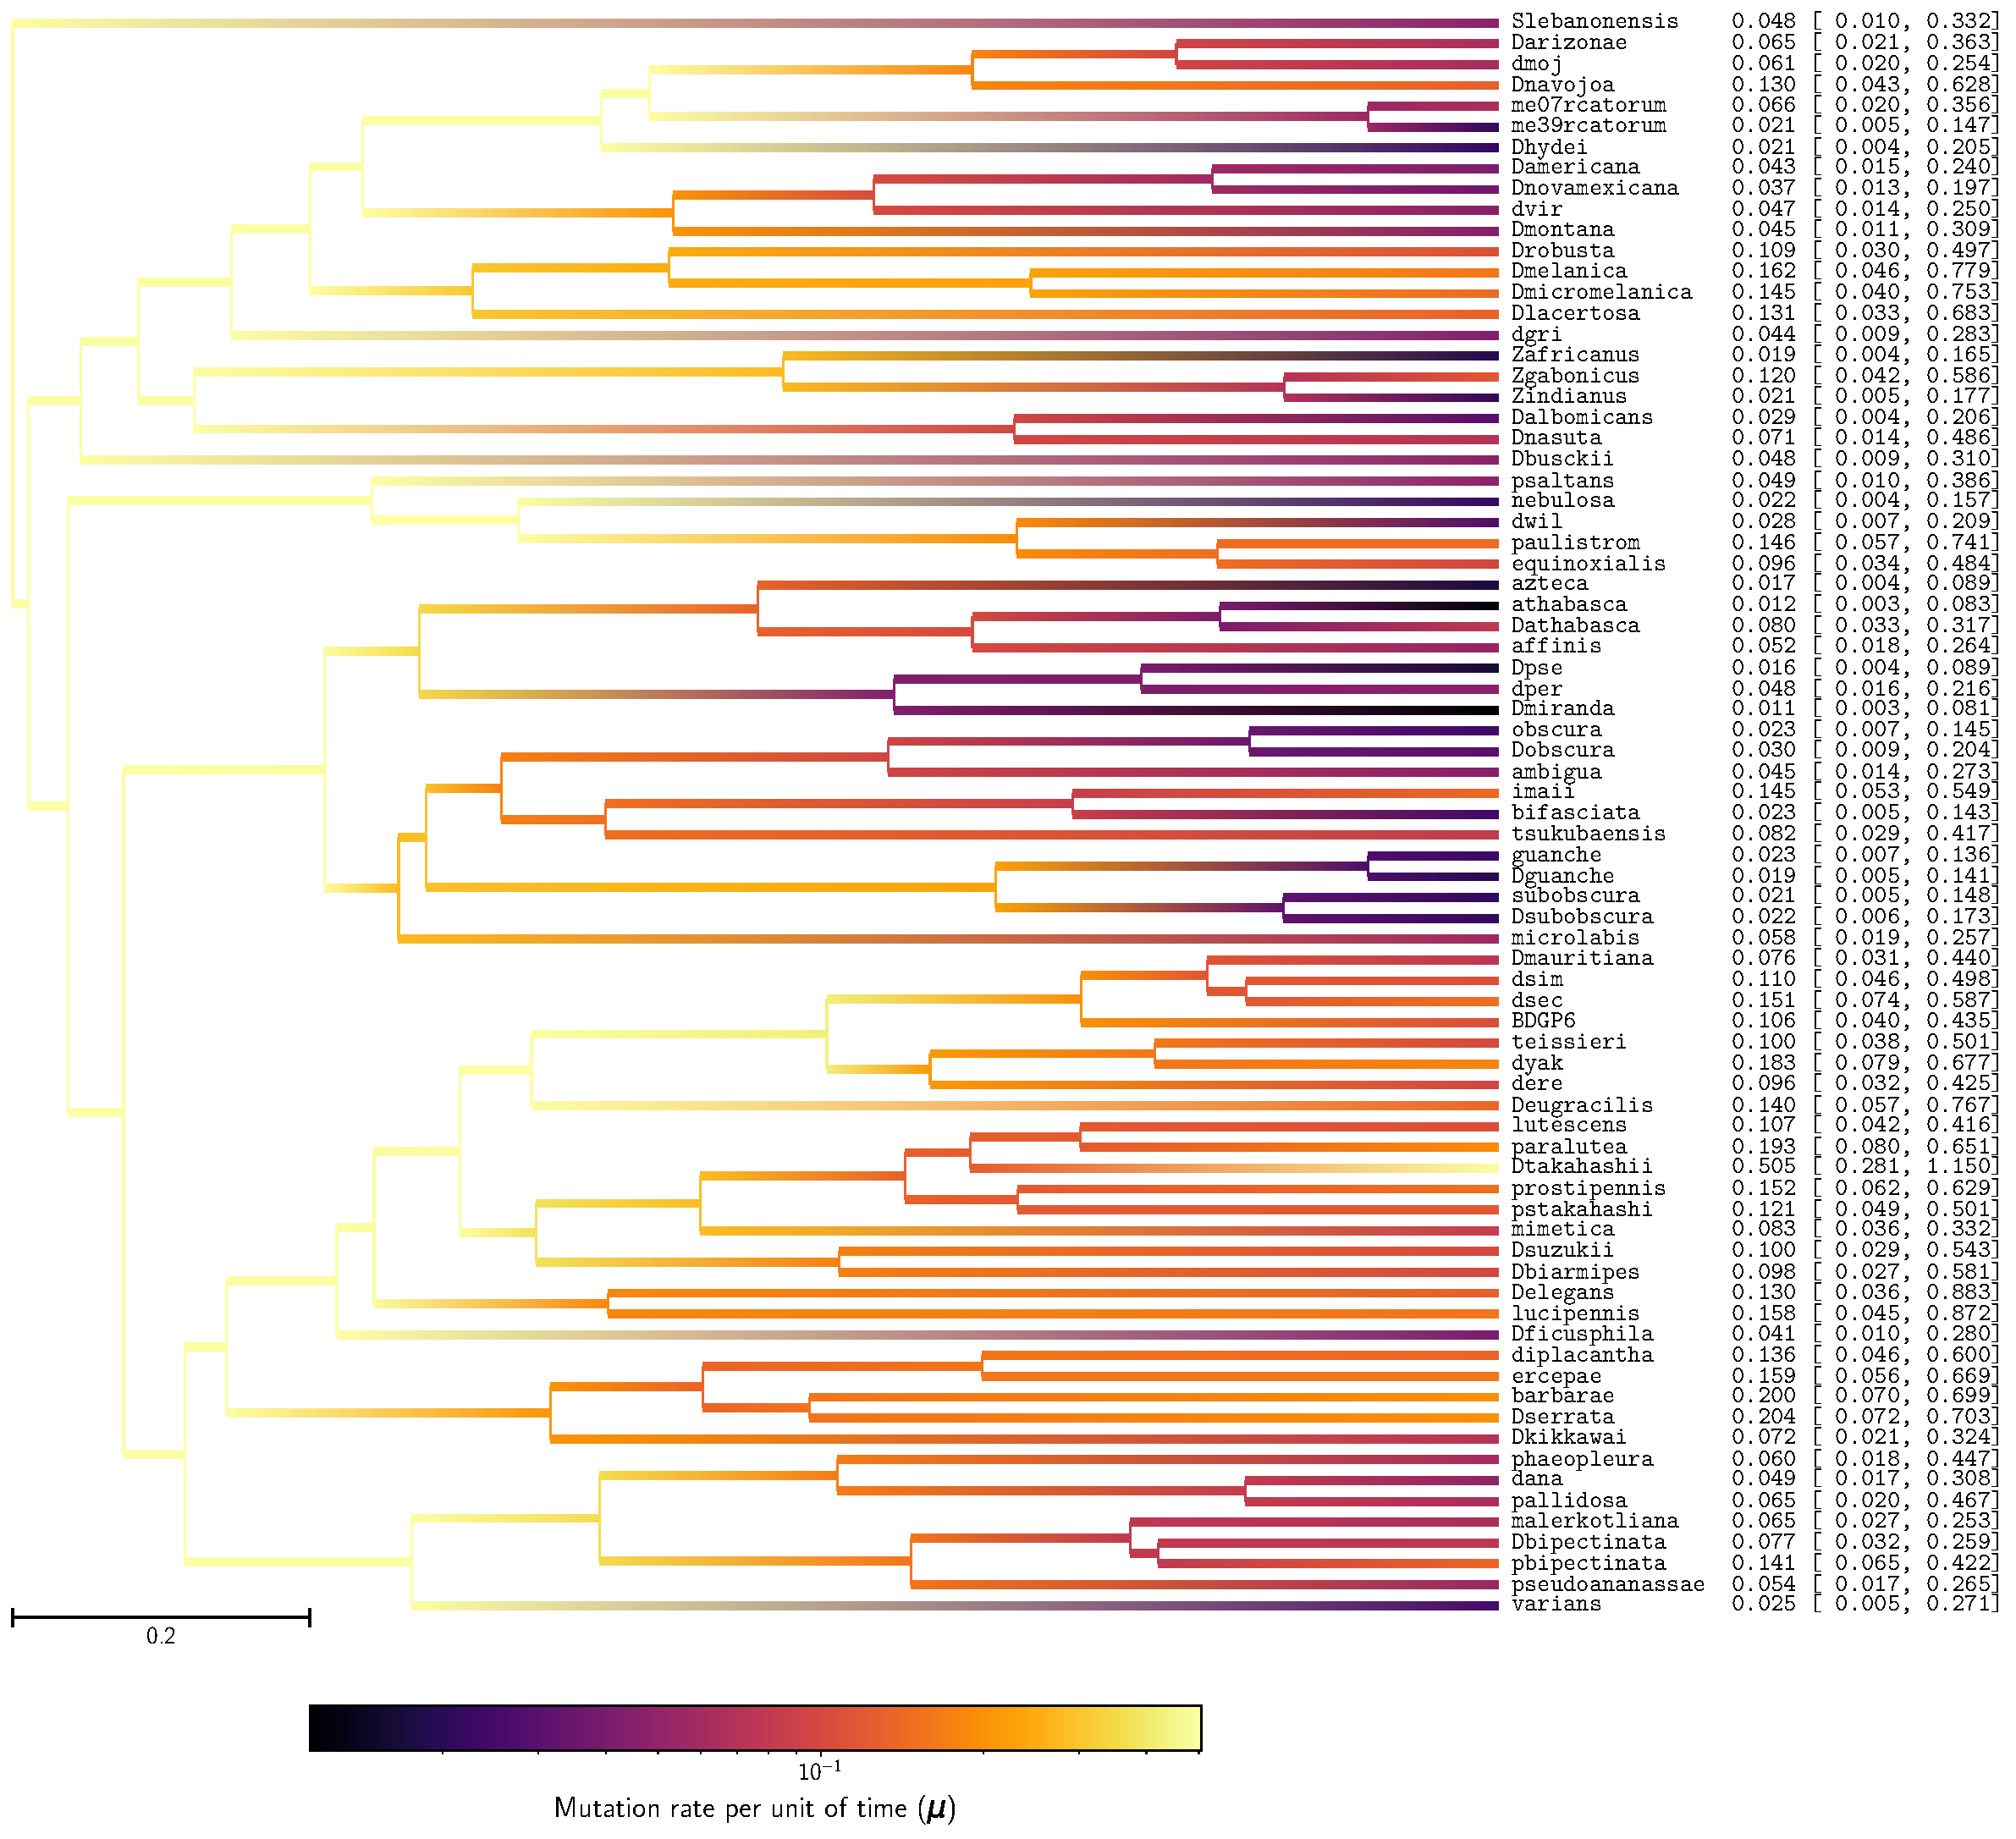
\includegraphics[valign=t, width=\linewidth, page=1, clip, trim=0cm 4.48cm 15.35cm 0cm]{mammals/18CDS_SiteMutSelBranchNe_R1_LogMutationRatePerTime}}
        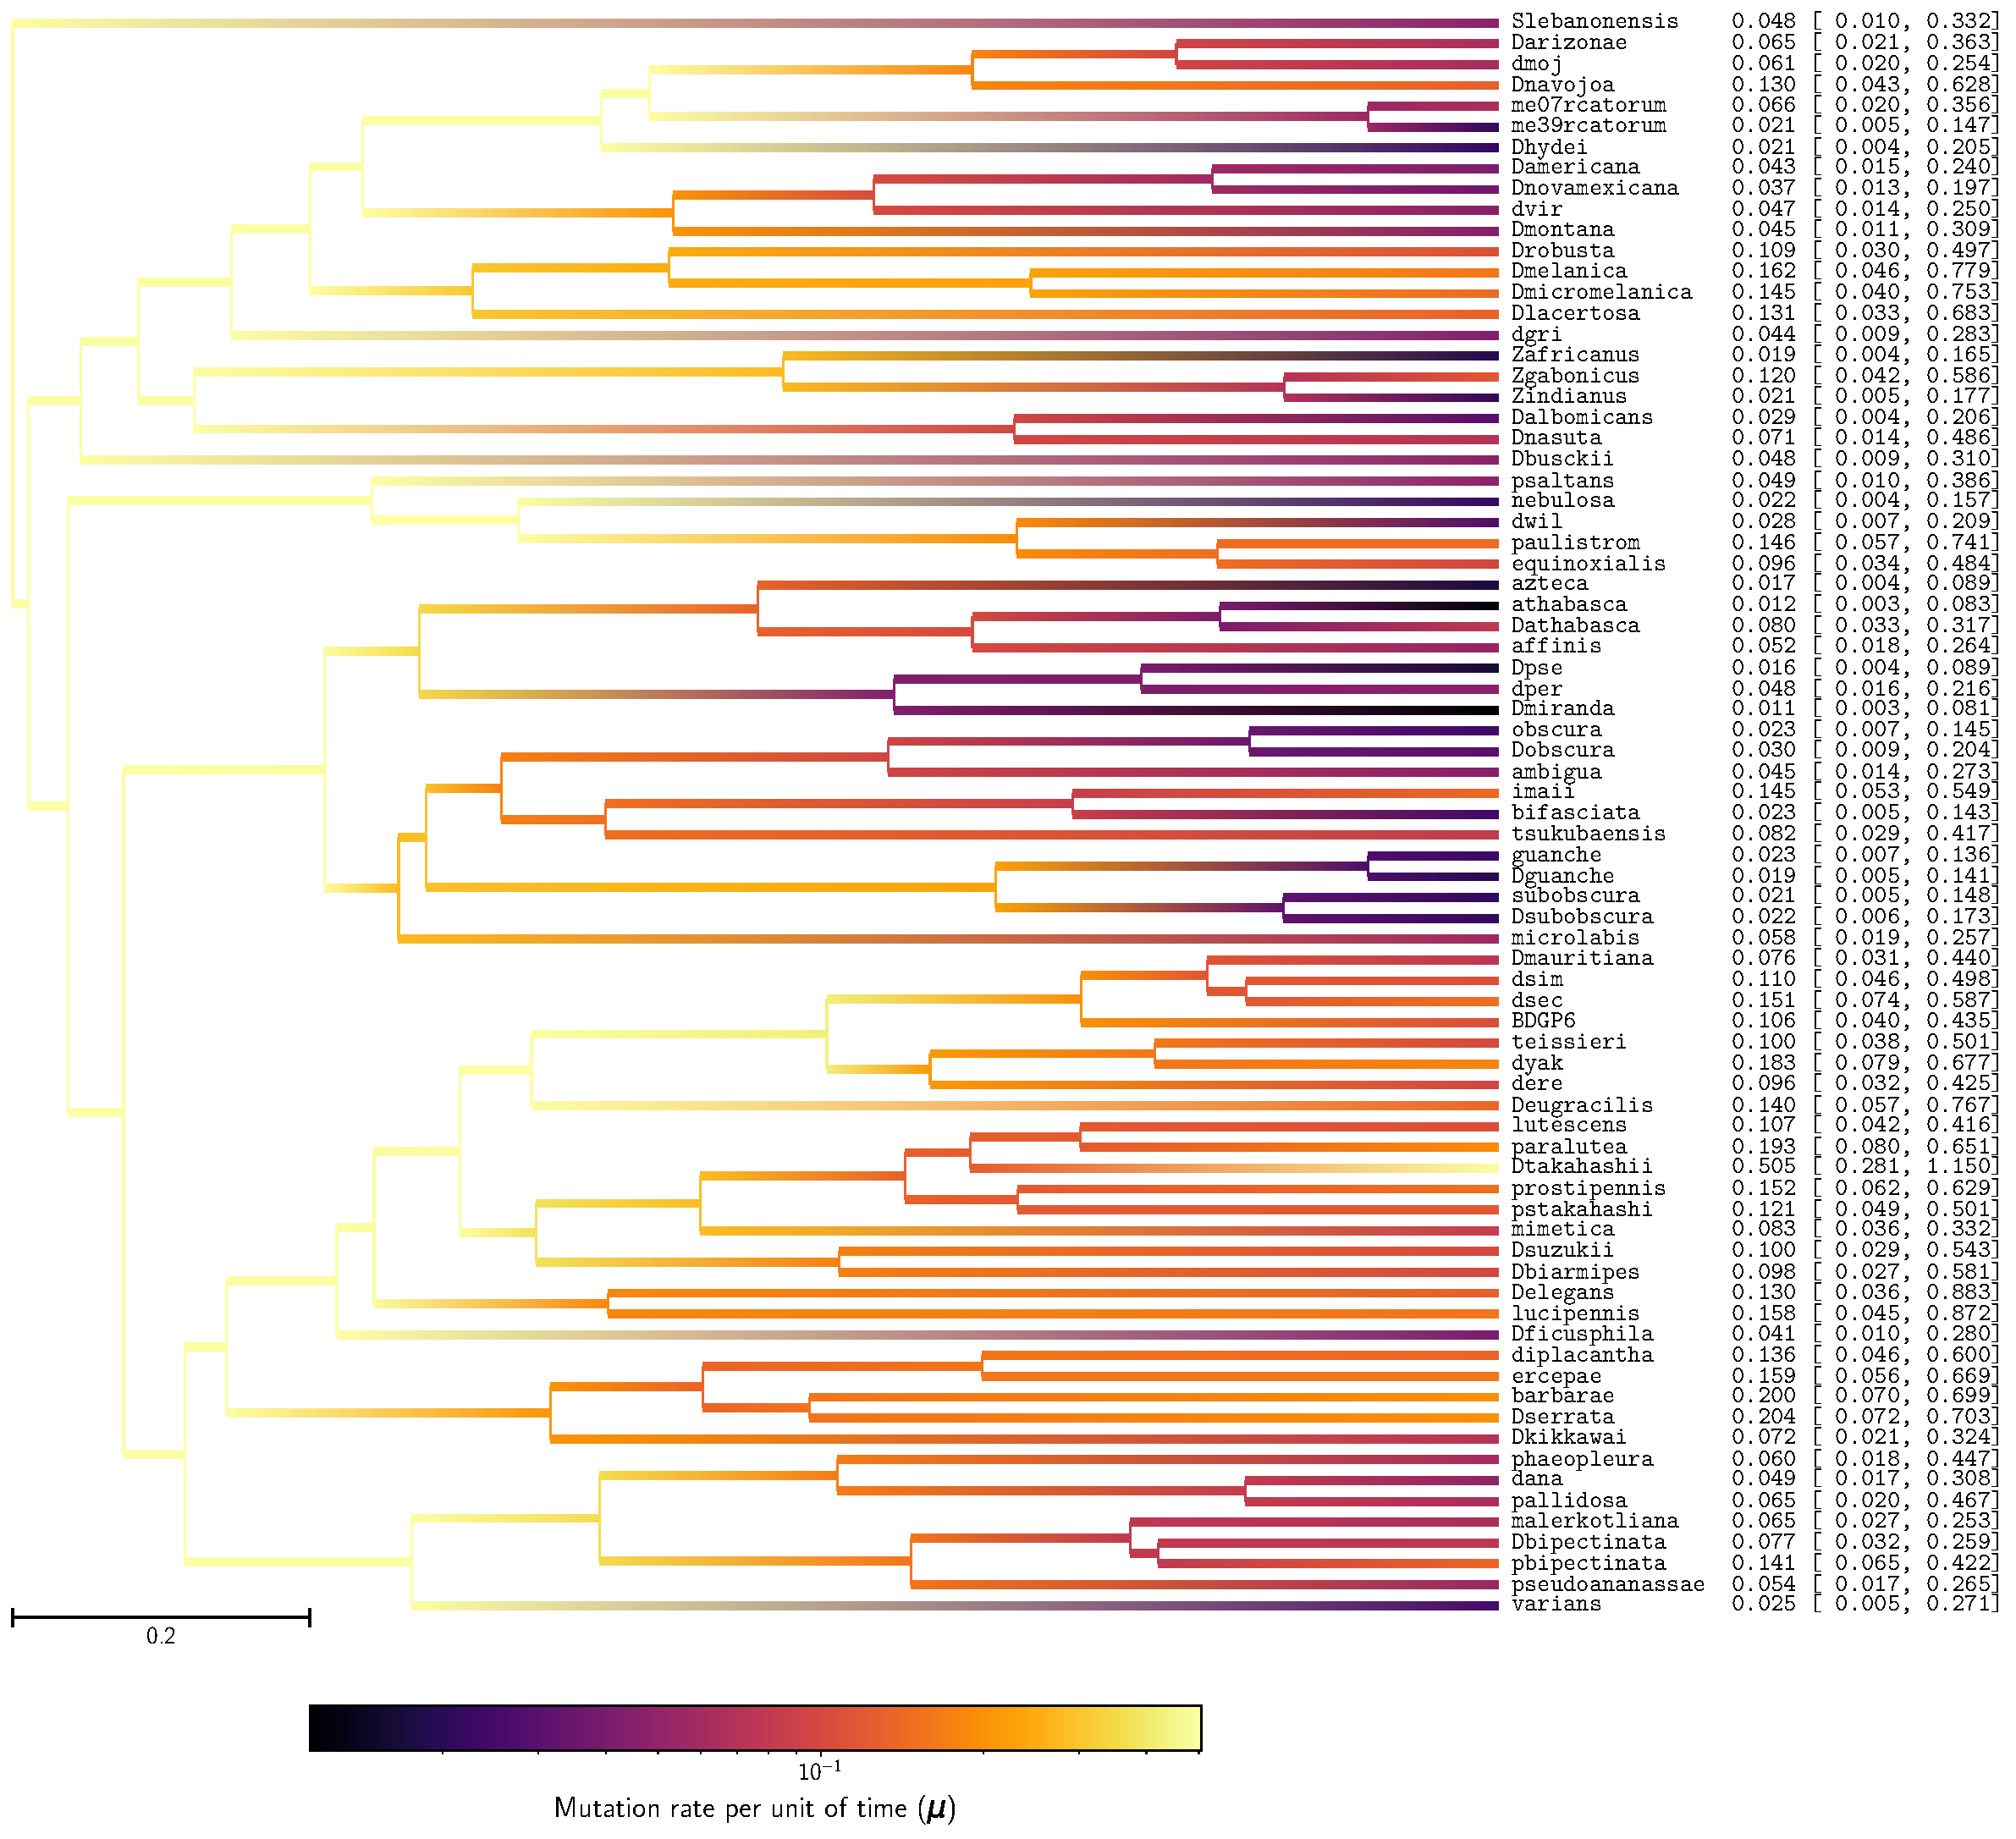
\includegraphics[valign=b,width=\linewidth, page=1, clip, trim=0cm 0cm 15.35cm 32.3cm]{mammals/18CDS_SiteMutSelBranchNe_R1_LogMutationRatePerTime}
    \end{minipage}
    \caption[Example of inferred $\Ne$ and $\mu$ on placental mammals dataset]{
    Example of inferred $\Ne$ and $\mu$ on placental mammals dataset.
    Inferences were performed on a randomly chosen set of $18$ coding sequences (\acrshort{CDS}) out of $226$ highly conserved CDS~($<1\%$ of gaps).
    Only highly conserved \acrshort{CDS} were retained such that the assumption of constant fitness landscape is not incautiously broken by protein with changing function and/or adaptive selection.
    Brownian processes along the tree are represented for effective population size~($\Ne$, left panel) and mutation rate per site per unit of time~($\mu$, right panel).
    Mean values of \acrshort{MCMC} (after burn-in) are obtained at each node of the tree, hence a gradient can be extrapolated along each branch.
    At each node, the inner circle represents the lower bound of the \acrshort{MCMC} $90\%$ confidence interval, and the outer circle represent the upper bound, as to give visual input into the range of estimation.
    $\mu$ spanned almost $2$ order of magnitude, and if we assume the root to be $105$My old~\citep{Kumar2017}, the rescaled mutation rate per site per year in extant species is between $\smash{1.1e^{-10}}$ and $\smash{7.8e^{-9}}$.
    $\Ne$ at the root of the tree is arbitrarily set to $1$, and all values are relative to the root.
    }
    \label{fig:mammals_popsize_and_mutrate}
\end{figure}

We reconstructed long-term changes of effective population size~($\Ne$) and mutation rate per site per unit of time~($\mu$) in placental mammals, with alignments extracted from OrthoMam database~\citep{Ranwez2007,Scornavacca2019}.
Life-history traits (\acrshort{LHT}) for longevity, age at maturity and weight were obtained from AnAge database~\citep{DEMAGALHAES2009,Tacutu2012}.
We focused our analysis on 77 taxa for which information is available for at least one \acrshort{LHT}.

In the result of this analysis, depicted in figure~\ref{fig:mammals_popsize_and_mutrate}), we visually observe a global trend of increased $\Ne$ throughout the tree around $90$ and $60$ My.
We also observe $\Ne$ to be lower in \textit{Cetacea} and \textit{Camelidae}, while being higher in \textit{Rodentia} and \textit{Pecora}.
In some clades we can see a decrease along a single branch of the tree, for example \textit{Heterocephalus glaber} or \textit{Acinonyx jubatus}.

The analysis of the covariance matrix presented in table~\ref{fig:mammals_correlation}, discarding phylogenetic inertia, shows that $\Ne$ is positively correlated~($r^2 = 0.44$) with the mutation rate per unit of time, which is compatible with the assumption that large population are small-sized and with a shorter generation time.
Moreover the effective population size is negatively correlated with longevity, age at maturity and weight (Table~\ref{fig:mammals_correlation}), consistent with the observation that larger population have small-sized and short-lived individuals~\citep{Galtier2016,Romiguier2014}.
The partial-correlation coefficients (see definition section~\ref{subsec:partial-correlation-coefficient} and table~\ref{tab:table-partcor-mammals} in supplementary materials) are not significantly different from $0$.

However, if the trend of $\Ne$ would be in the right direction, the magnitude of inferred $\Ne$ is vastly underestimated by our method, with a ratio of $2.5$ between the maximum and minimum $\Ne$ in extant species (see figure~\ref{fig:mammals_popsize_and_mutrate}).
To assess the reproducibility of our inference, we analysed a concatenated random sample of $18$ highly conserved coding sequences~($\leq 1\%$ of gaps in the alignment), and repeated the procedure on different random samples of $18$ \acrshort{CDS}.
Overall the estimation of $\Ne$ is reproducible for a random subset of \acrshort{CDS}, as depicted in figure~\ref{fig:mammals_repeatability}.

We performed other empirical experiments using a group of isopod species that have made multiple independent transitions to subterranean environments.
Protein coding \acrshort{DNA} sequences alignment and qualitative life-history traits such as habitat (surface or underground), pigmentation (depigmented, partially depigmented or pigmented) and ocular structure (anophthalmia, microphthalmia, or ocular) are available for these species~\citep{Saclier2018}.
Estimation of $\Ne$ reveals a correlation between qualitative life-history traits and $\Ne$, presented section~\ref{sec:empirical-data-in-isopods} in supplementary materials.
However, these correlations are sensitive to phylogenetic inertia since multivariate log-Brownian does not accommodate qualitative traits, although this particular dataset is composed of surface and subterranean species reducing biases.

Additionally, our empirical framework was also applied in primates (see~\ref{sec:empirical-data-in-primates} and in supplementary materials).
Reconstructed $\Ne$ and $\mu$ are related to \acrshort{LHT} (mass, female maturity, generation time and longevity), synonymous diversity ($\ps$) and non-synonymous over synonymous ($\pnps$).
Finally, our empirical framework was also applied in drosophila and related to genome size (see~\ref{sec:empirical-data-in-drosophila} and in supplementary materials).
These experiments however did not uncover statistically significant correlation between $\Ne$ and life-history traits.

\begin{table}[htbp]
    \centering
\noindent\adjustbox{max width=\textwidth}{%
\begin{tabu}{|c||c|c|c|}
\hline
\textbf{Correlation ($\bm{\rho}$)} & $\bm{N_{\mathrm{e}}}$ & $\bm{\mu}$ & \textbf{LogGenomeSize}\\
\hhline{|=#=|=|=|}
$\bm{N_{\mathrm{e}}}$ & - & $-0.0623$ & $-0.144$\\\hline
$\bm{\mu}$ & - & - & $0.224$\\\hline
\textbf{LogGenomeSize} & - & - & -\\\hline
\end{tabu}}

    \caption[Traits correlation]{
    Correlation coefficient between effective population size~($\Ne$), mutation rate per site per unit of time~($\mu$), and life-history traits (Maximum longevity, adult weight and female maturity), taking account phylogenetic inertia.
    Correlation coefficients are between $-1$ and $1$.
    Asterisks indicate strength of support of the posterior probability to be different than $0$ (pp) as $\smash{^{*}} pp > 0.95$ and $\smash{^{**}} pp > 0.975$.
    Observed correlations are compatible with the interpretation that large populations are composed of small, short-lived individuals.
    Moreover if the mutation rate per generation is considered constant in first approximation, the mutation rate per unit of time is positively correlated to generation rate, hence to population size.
    }
    \label{fig:mammals_correlation}
\end{table}


\section{Discussion}
\label{sec:Discussion}
% Summary 
Mechanistic phylogenetic codon models explicitly define the substitution rates as function of the mutation rate, selection and genetic drift.
Applied on an alignment of \acrshort{DNA} coding sequence, the mechanistic model can estimate amino-acid fitness landscapes along the \acrshort{DNA} sequence.
On the other hand, molecular comparative framework reconstruct the joint evolution of life history, molecular and population-genetics traits along the phylogeny, intrinsically including phylogenetic inertia.
Combined together, the resulting framework can reconstruct site-heterogeneous amino-acid fitness landscapes, estimates the age of internal nodes, and finally reconstitute branch-heterogeneous life-history traits, mutation rate ($\mu$) and effective population size ($\Ne$), with their correlation.
Testing the method against simulated alignments suggests the signal is strong enough in protein-coding \acrshort{DNA} alignment to infer selection at the site level, and long-term changes in $\Ne$ and $\mu$ using a phylogenetic approach.
In placental mammals, $\Ne$ correlates negatively with longevity, weight and maturity, and positively with $\mu$.
Our observations suggest that the empirical signal is strong enough such that we can infer the directional trends in changes.

% Longvariance in Ne 
If the trend of variations in $\Ne$ is in right direction, the magnitude of change across the phylogeny with a ratio of $2.5$ is greatly inferior to the expected variation observed in mammals~\citep{Galtier2016, Brevet2019}.
Different mechanisms not accounted for by the model could explain such a low variation of reconstructed $\Ne$.

First, genetic hitchhiking, Hill-Robertson interference, and short-term fluctuations of $\Ne$ could generate this effect.
However, inference made on alignments simulated by Wright-Fisher model accounting for linkage tends to show that this effect is not strong enough in the regimes explored.

Second, $\mu$ and $\Ne$ could also be fluctuating along the genome.
This assumption needs to be tested, though we expect that relaxing this assumption would not change drastically the magnitude of inferred $\Ne$ since some of this fluctuation is absorbed by site-specific fitness profiles.

Third, the \acrshort{DNA} sequences could also be misaligned in some sites.
However we observe the same magnitude of inferred $\Ne$ for different set of genes indicating this might not be the primary reason.

Fourth, the genes selected in our alignments could be under adaptive evolution, or their function could have changed.
More precisely, the fitness profile at each site could change with time, either due to Red-Queen dynamics or due to epistasis because amino-acid substitutions occurred at other sites.
Simulation of \acrshort{DNA} coding sequences under an epistatic landscape seemingly points to epistasis being the principal factor to be investigated, since $\Ne$ could not be appropriately estimated in such a case.
Independently, the magnitude of inferred $\Ne$ is quite similar for the placental mammals dataset and the primates dataset, while we would expect a greater discrepancy at longer phylogenetic scale.
An explanation could be that epistasis is more prevalent at longer time-scale, because the total number of substitutions from root to leaves is greater, hence the fitness landscape is less stable.
Thought modelling epistasis in an inference framework is a complex biological, mathematical and computational problem, this work points to a potential signal of epistasis that could be retrieved in phylogenetic context.
% None equilibrium properties

% Perspective : codon bias
Our model also assumes no bias in codon usage, though the strength of selection for a particular codon (or set of codons) among all synonymous possible codons has been proved to be substantial~\citep{Yang2008,Plotkin2011}.
This assumption can be relaxed by implementing codon preferences that are shared across all sites such that $41$ more parameters would be required in total.
Such implementation would provide the advantage of estimating codon usage biases, and of accounting for its confounding effect while estimating selection and $\Ne$.

% Perspective: 
Bayesian computations shown in this study are based on relatively small alignments ($20,000$ sites at most), and with a limited parametrization in the number of fitness profile categories~($50$).
Analysing execution duration of the program (not shown) leads to conclude that the number of fitness profile categories is the limiting step to expand the computation.
To estimate a more statistically stable genome-wide $\Ne$, we could develop an extended version leveraging parallel computing, where each coding sequence has its own computing process and own profile categories, but the $\Ne$ would be shared by all computing processes.
By increasing the number of categories per gene, the magnitude of inferred $\Ne$ would also increase, since fitness profiles would be sharper.

% Perspective: increase power
Mutation-selection models originated with the aim of increasing the power to detect adaptive evolution, by modelling explicitly the confounding effect of purifying selection.
However, by assuming constant $\Ne$ along a phylogeny, the statistical power to detect sites under adaptive evolution is not optimal.
Fitness profiles estimated are averaged along the phylogeny and are more seemingly neutral than our estimated profiles under our present framework (see section~\ref{subsec:fitness-profile-entropy} and table~\ref{tab:table-entropy-aa-mutselne} in supplementary materials).
Even though our method requires more computing resources to estimate fitness profiles, it provides a better null model of purifying selection to test against the presence of adaptive evolution.

% Comparison with other methods
Other methods have recently been developed to reconstruct phylogenetic changes in $\Ne$.
For example, a method recently developed by \citet{Brevet2019} uses \acrshort{DNA} coding sequences, a distribution of fitness effects, polymorphism and generation time for some present-day species to reconstruct $\Ne$ along the phylogeny~\citep{Brevet2019}.
This method also based on the quasi-neutral theory of evolution allows to estimate the absolute value of $\Ne$, even for species where the polymorphism is unavailable.
Here our method requires neither generation time nor polymorphism, and the fitness effects are not constrained to a specific distribution.
However, the inferred values are solely relative and the computation requires more computing resources.

% Perspective: Short and long-term Ne
Estimating $\Ne$ in a mutation-selection phylogenetic model relies on the relation between $\Ne$ and relative strength of drift, where ultimately the signal of drift comes from the relative rate of substitutions.
However, they do not leverage a second aspect of $\Ne$ at the population level, which determines the neutral genetic diversity that can be maintained~($\pi=4\Ne \mu \tau$, where $\tau$ is the generation time).
Hence, polymorphic data give us independent empirical estimates of $\Ne$, based on the assumption that mutations are neutral.
In principle, our mechanistic model could be extended to leverage polymorphism within species in the case of differential selection, a method which has been previously pioneered in the case of $3$ species and using a distribution of fitness effect~\citep{Wilson2011}.
More generally, the nearly-neutral theory of evolution defines a long-term $\Ne$, which might be different from the short-term definition of $\Ne$~\citep{Platt2018}.
Thus we could ask if empirical independent estimations of $\Ne$ from within species (polymorphic diversity) and between species (substitutions) are congruent, and if not what are the mechanisms responsible for this discrepancy.

% Relation to ecology
Notwithstanding theoretical considerations on the quasi-neutral theory of evolution, empirical clues about the long-term trends in the direction of genetic drift, and changes between species allows to open a large diversity of ecological and evolutionary questions.
Spatial and temporal changes of genetic drift along ecological niches and events can be investigated to disentangle the underlying evolutionary and ecological pressures.

\begin{figure}[htbp]
    \centering
    \begin{minipage}{0.32\linewidth}
        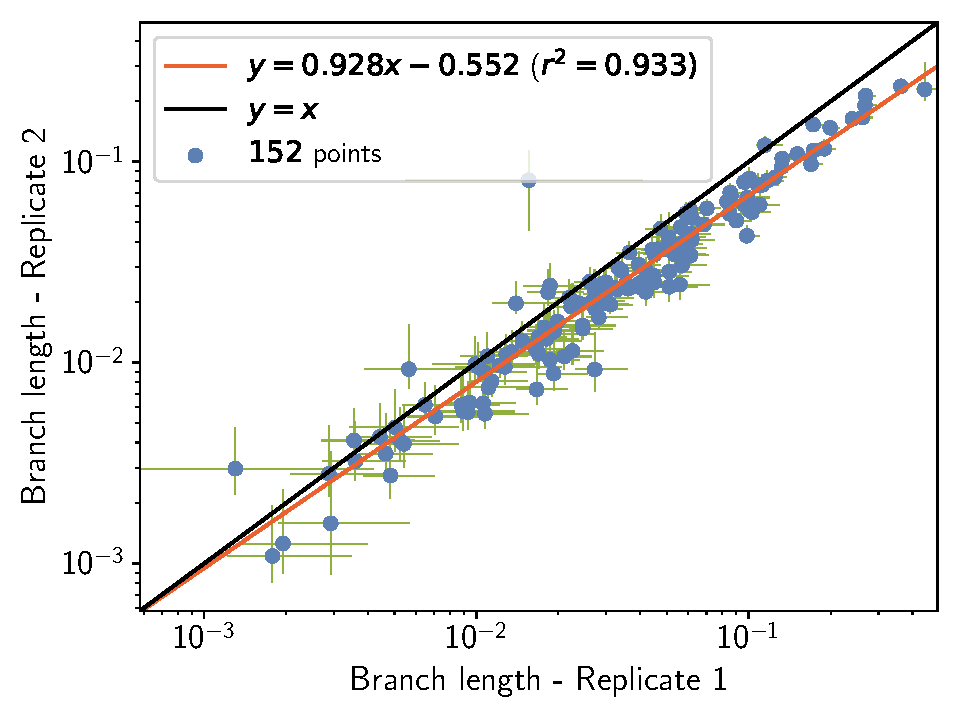
\includegraphics[width=\linewidth, page=1]{mammals/18CDS_SiteMutSelBranchNe_Rep_Log10BranchLength-1-2}
    \end{minipage}
    \llap{\raisebox{-1.1cm}{\scriptsize A\hspace{0.35cm}}}\hfill
    \begin{minipage}{0.32\linewidth}
        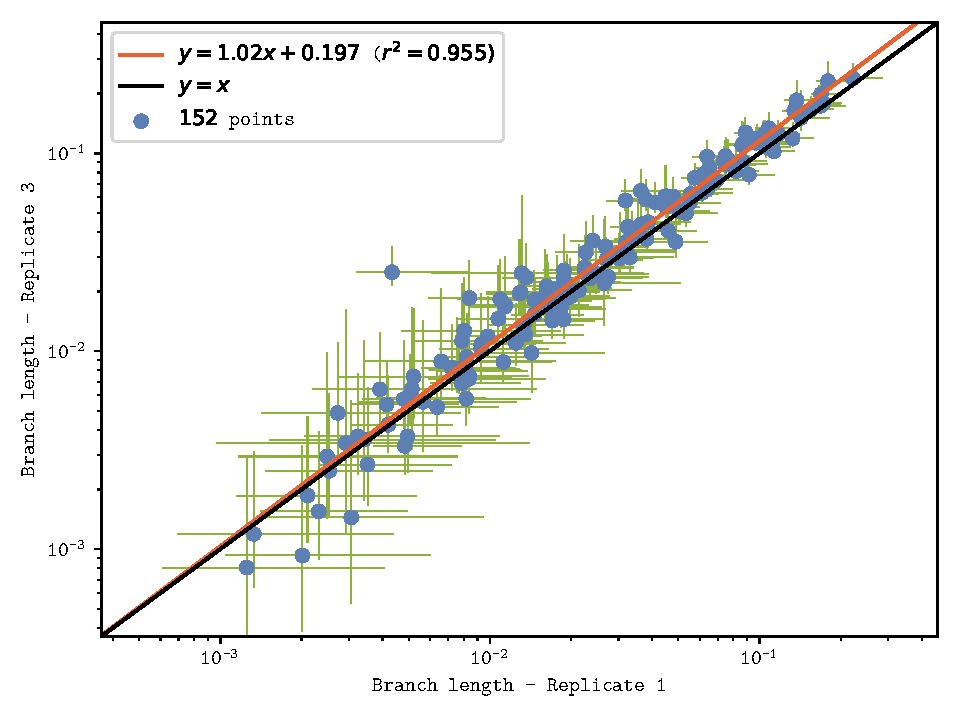
\includegraphics[width=\linewidth, page=1]{mammals/18CDS_SiteMutSelBranchNe_Rep_Log10BranchLength-1-3}
    \end{minipage}
    \llap{\raisebox{-1.1cm}{\scriptsize B\hspace{0.35cm}}}\hfill
    \begin{minipage}{0.32\linewidth}
        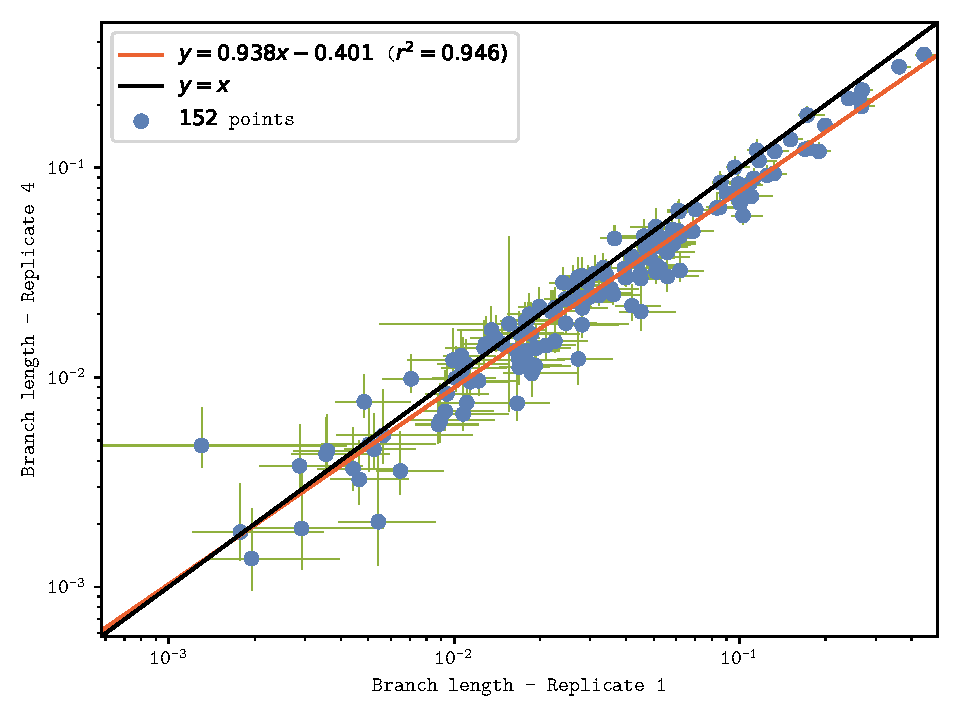
\includegraphics[width=\linewidth, page=1]{mammals/18CDS_SiteMutSelBranchNe_Rep_Log10BranchLength-1-4}
    \end{minipage}
    \llap{\raisebox{-1.1cm}{\scriptsize C\hspace{0.35cm}}}\hfill
    \begin{minipage}{0.32\linewidth}
        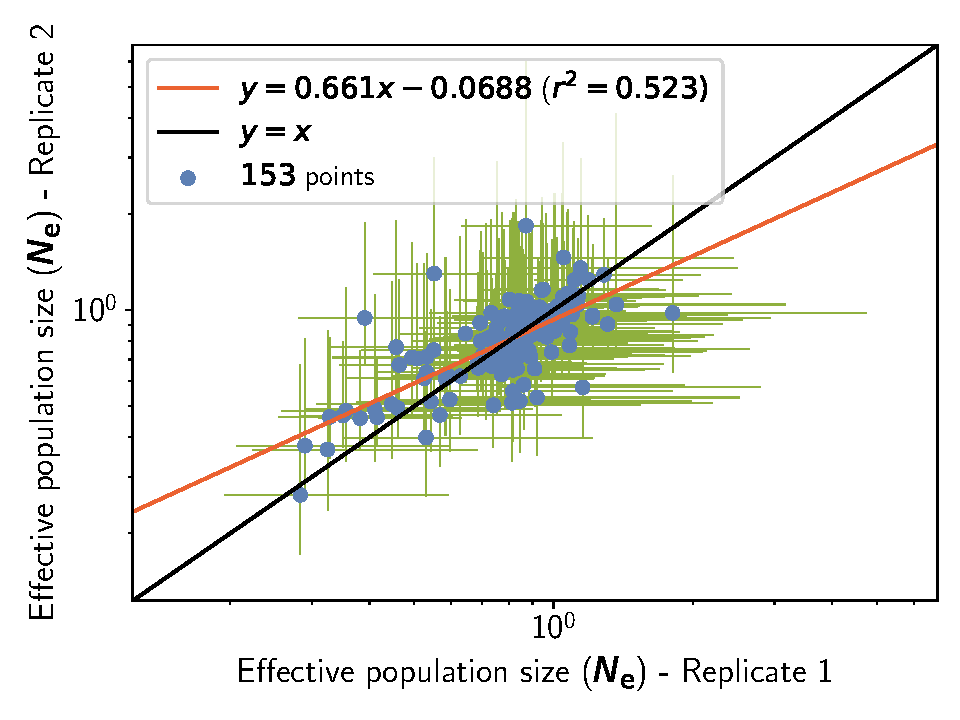
\includegraphics[width=\linewidth, page=1]{mammals/18CDS_SiteMutSelBranchNe_Rep_LogPopulationSize-1-2}
    \end{minipage}
    \llap{\raisebox{-1.1cm}{\scriptsize D\hspace{0.35cm}}}\hfill
    \begin{minipage}{0.32\linewidth}
        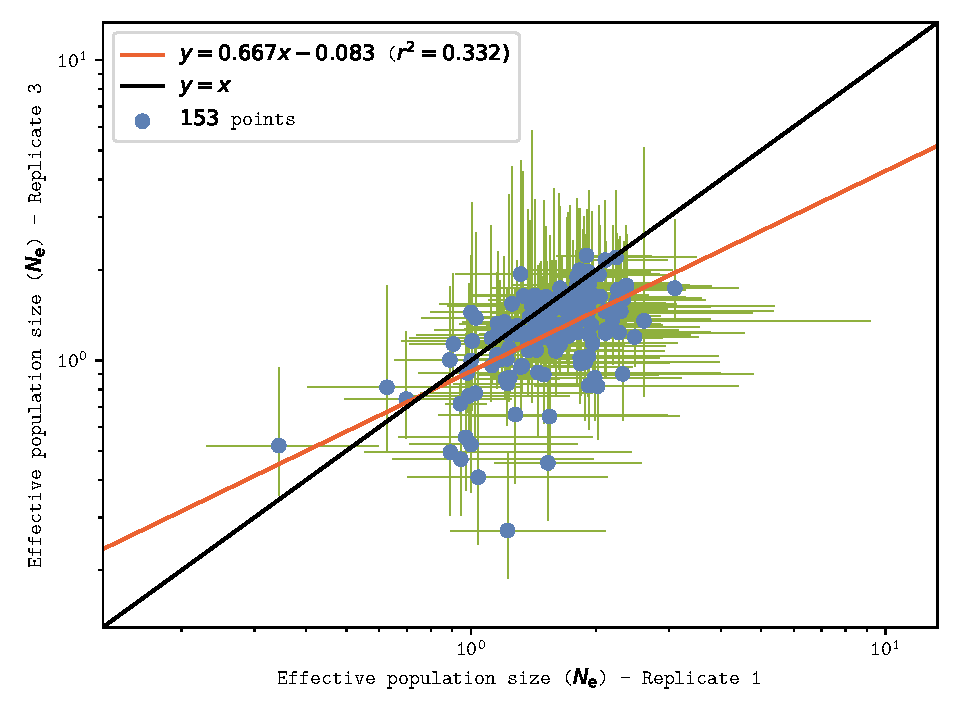
\includegraphics[width=\linewidth, page=1]{mammals/18CDS_SiteMutSelBranchNe_Rep_LogPopulationSize-1-3}
    \end{minipage}
    \llap{\raisebox{-1.1cm}{\scriptsize E\hspace{0.35cm}}}\hfill
    \begin{minipage}{0.32\linewidth}
        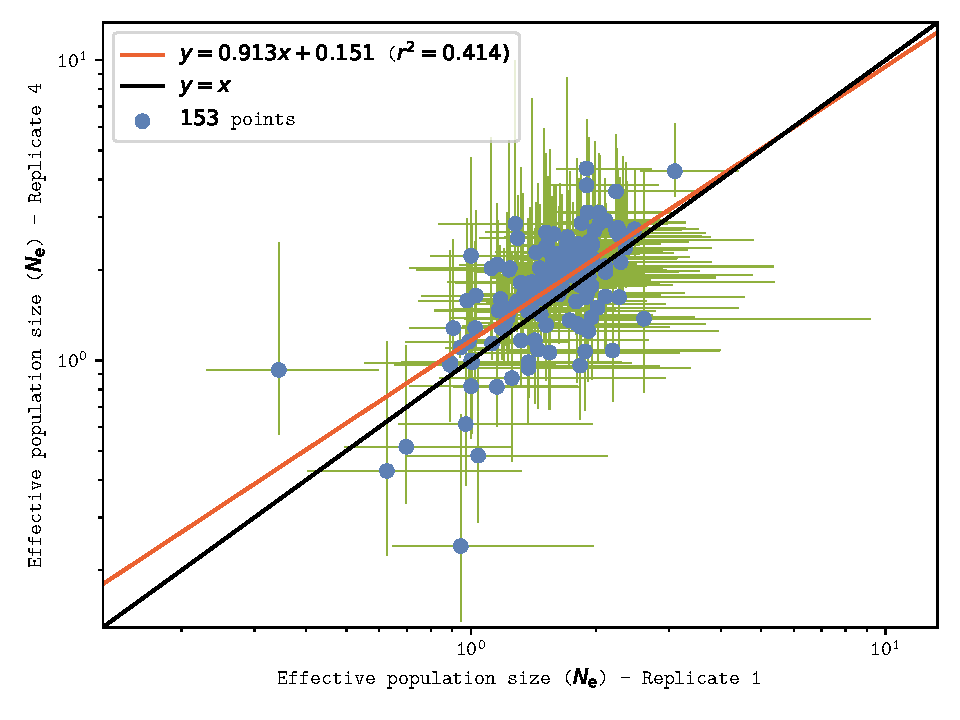
\includegraphics[width=\linewidth, page=1]{mammals/18CDS_SiteMutSelBranchNe_Rep_LogPopulationSize-1-4}
    \end{minipage}
    \llap{\raisebox{-1.1cm}{\scriptsize F\hspace{0.35cm}}}\hfill
    \caption[Repeatability of experiments]{
    Repeatability of experiments.
    $3$ independent inferences were performed on a randomly chosen set of $18$ coding sequences (\acrshort{CDS}) out of $226$.
    Each plot is a correlation between a pair of experiments for a given parameter.
    Mutation rate per unit of time~($\mu$), is represented in the top row (panels A, B and C), while effective population size~($\Ne$) is represented in the bottom row (panels D, E and F).
    For each node of the tree, the mean posterior of the parameter~($\Ne$ or $\mu$) over the \acrshort{MCMC} (after burn-in) is represented in blue dots, green solid lines are the $90\%$ confidence interval of the \acrshort{MCMC}.
    Solid red line is the regression line between experiments.
    Inference of $\mu$ is more reproducible than $\Ne$, but overall the experiment is reproducible for a random subset of \acrshort{CDS}.
    }
    \label{fig:mammals_repeatability}
\end{figure}


\section{Materials and Methods}
\label{sec:MatMet}
The parameterization of the models is described as a Bayesian hierarchical model, containing the prior distributions and parameters of the model.
This hierarchical model is formally represented as directed acyclic graph, depicted in figure~\ref{fig:DAG-MutSelNe}.

\subsection{Nucleotide mutation rates}
The generalized time-reversible nucleotide mutation rate matrix $\Mutmatrix$ is a function of the nucleotide frequencies $\Mutequi$ and the symmetric exchangeability rates $\Exchan$~\citep{Tavare1986}.
$\Mutequi = (\mutequi_A , \mutequi_C , \mutequi_G , \mutequi_T)$ is the equilibrium base frequency vector, giving the frequency at which each base occurs at each site.
$\Exchan = \left( \exchan_{AC}, \exchan_{AG}, \exchan_{AT}, \exchan_{CG}, \exchan_{CT}, \exchan_{GT}\right)$ is the vector of exchangeabilities between nucleotides.
Altogether, the rate matrix is:
\begin{equation}
    \label{eq:gtr-mutrates}
    \Mutmatrix =
    \begin{pmatrix}
        - & {\exchan_{AC}\mutequi_C} & {\exchan_{AG}\mutequi_G} & {\exchan_{AT}\mutequi_T} \\
        {\exchan_{AC}\mutequi_A} &                        - & {\exchan_{CG}\mutequi_G} & {\exchan_{CT}\mutequi_T} \\
        {\exchan_{AG}\mutequi_A} & {\exchan_{CG}\mutequi_C} &                        - & {\exchan_{GT}\mutequi_T} \\
        {\exchan_{AT}\mutequi_A} & {\exchan_{CT}\mutequi_C} & {\exchan_{GT}\mutequi_G} & -
    \end{pmatrix}
\end{equation}
By definition, the sum of the entries in each row of the nucleotide rate matrix $\Mutmatrix$ is equal to $0$, giving the diagonal entries:
\begin{equation}
    \mutmatrix_{a,a} = - \sum\limits_{ b \neq a} \mutmatrix_{a,b}
\end{equation}
The prior on the exchangeabilities $\Exchan$ is a uniform Dirichlet distribution of dimension $6$:
\begin{equation}
    \label{eq:DistribExchan}
    \Exchan \sim \text{Dir}\left( \dfrac{1}{6} , 6\right).
\end{equation}
The prior on the equilibrium base frequencies $\Mutequi$ is a uniform Dirichlet distribution of dimension $4$:
\begin{equation}
    \label{eq:DistribMutequi}
    \Mutequi \sim \text{Dir}\left( \dfrac{1}{4} , 4\right)
\end{equation}
The general time-reversible nucleotide matrix is normalized such that the total flow equals to $1$:
\begin{equation}
    \sum\limits_{a \in \{A, C, G, T\}} - \mutequi_a \mutmatrix_{a,a} = 1.
\end{equation}

\subsection{Site-dependent selection}
\label{sec:profiles}
For each category $\Setcat$, a $20$-dimensional fitness profile $\Profile\catexp$ (summing to $1$) is distributed as a Dirichlet of center $\centerProfile$ and concentration $\concentrationProfile$:
\begin{equation}
    \label{eq:DistribBase}
    \Profile\catexp \sim \text{Dir}\left( \centerProfile,\ \concentrationProfile \right),\ \Setcat.
\end{equation}
For an alignment of size $\Nsite$, each site $\Setsite$ is assigned a fitness profile category of amino acids $\catsite \in \catInterval $.
The total number of sites falling in each fitness profile category $\cat$ is denoted $\catmultivar_{\cat}$.
The $\Ncat$-dimensional vector $\catMultiVar$ is distributed as a multinomial of event probabilities $\StickBreaking$:
\begin{align}
    \label{eq:DistribMultinomial}
    \catMultiVar \sim \text{Multinomial}\left( \StickBreaking \right).
\end{align}
The event probabilities $\Ncat$-dimensional vector~($\StickBreaking$) of falling into each category is distributed as a stick-breaking \gls{Dirichlet process}:
\begin{align}
    \label{eq:DistribStickBreaking}
    \begin{split}
        & \StickBreaking \sim \text{StickBreaking}\left( \Ncat, \stickbreakinghyper \right)\\
        \iff & \stickbreaking_{\cat} = \stick_{\cat}\cdot \prod _{{\indice=1}}^{{\cat-1}}\left(1-\stick_{\indice}\right),\ \Setcat,
    \end{split}
\end{align}
where $\stick_{\cat}$ are i.i.d.
from a beta distribution
\begin{equation}
    \label{eq:Beta}
    \stick_{\cat} \sim \text{Beta}\left( 1, \stickbreakinghyper \right),\ \Setcat.
\end{equation}
The Malthusian fitness selection coefficients $\Fit\siteexp$ at site $\site$, are obtained by taking the logarithm of the fitness profile assigned to this site:
\begin{equation}
    \label{eq:sitefitness}
    \Fit\siteexp = \ln \left( \Profile^{\left( \catsite \right)} \right),\ \Setsite.
\end{equation}

\subsection{Dated tree}
The topology of the rooted phylogenetic tree is supposed to be known and is not estimated by the model.
The model estimates the dates at which branches split, thus the dated tree requires $\Ntaxa - 2$ internal node ages that are free parameters, where $\Ntaxa$ is the number of extant taxa (leaves of the tree).
The node ages $\age\nodeexp,\ \Setinternal$ are drawn uniformly such that a node cannot be younger than the oldest of its $2$ descendant children, and must also be younger than its parent:
\begin{equation}
    \label{eq:Distribage}
    \age\nodeexp \ \sim \mathcal{U}\left( \text{max}\left(\age^{(\text{children})} \right), \age^{(\text{parent})} \right)
\end{equation}
By definition, leaf ages are all set to $0$. The root age is set arbitrarily to $1$, but if fossils data are also available the dated tree can be rescaled into absolute time using cross-multiplication.\\
The duration of the branch~($\branchtime\branchexp$), for each branch $\Setbranch$ is defined as the difference in ages between the oldest node at the tip of the branch $\age^{(\nodeUp)}$, and the youngest node $\age^{(\nodeDown)}$:
\begin{equation}
    \label{eq:ageTobranchtime}
    \branchtime\branchexp = \age^{(\nodeUp)} - \age^{(\nodeDown)}.
\end{equation}

\subsection{Branch dependent traits}
The effective population size $\Ne$ and mutation rate per unit of time $\mu$ are assumed to evolve along the phylogeny, and to be correlated.
If quantitative life-history-traits (\acrshort{LHT}) are also available for some nodes of the tree (leaves and/or internal nodes), they are also assumed to evolve along the phylogeny and to be correlated between them, and with $\Ne$ and $\mu$.
The total number of traits (counting $\Ne$, $\mu$ and all user-defined LHT) is denoted $\Ntrait$.
Their fluctuations are modelled by a $\Ntrait$-dimensional log-Brownian process $\Brownian\nodeexp$ at each node $\Setnode$ of the tree, including the root and leaves.
The first dimension (indexed by $0$) of the log-Brownian contain $\Ne$, and the second dimension (indexed by $1$) contains $\mu$.
The log-Brownian process and variables of interest~($\mu$ and $\Ne$) are linked by an exponential transformation:
\begin{equation}
    \begin{dcases}
        \Ne\nodeexp = \e^{ \brownian_{0}\nodeexp } \\
        \mu\nodeexp = \e^{ \brownian_{1}\nodeexp },
    \end{dcases}
\end{equation}
where the effective population size at the root is set to $1$ for identifiability of the fitness profiles.
It is important to note that inferred correlation between $\Ne$, $\mu$ and other \acrshort{LHT} is thus in the log space, and that quantitative \acrshort{LHT} must be inputted in log scale.

Along a branch $\Setbranch$ of the tree, a log-Brownian process starts at the oldest node at the tip of the branch~($\nodeUp$), and ends at the youngest node~($\nodeDown$).
However we are interested in the average over the branch to define the codon substitution matrices along the branch.
In the case of log-Brownian process, the most likely path (or geodesic) from $\Brownian^{(\nodeUp)}$ to $\Brownian^{(\nodeDown)}$ is the straight line, and therefore, it would make sense to take the mean value of $\e^{\Brownian\nodeexp}$ along this geodesic.
We then have $\Ne\branchexp$ and $\mu\branchexp$ for each branch $\Setbranch$ of the tree:
\begin{equation}
    \label{eq:branchNemu}
    \begin{dcases}
        \Ne\branchexp = \dfrac{\e^{\brownian_{0}^{(\nodeDown)}} - \e^{\brownian_{0}^{(\nodeUp)}}}{\brownian_{0}^{(\nodeDown)} - \brownian_{0}^{(\nodeUp)}} \\
        \mu\branchexp = \dfrac{\e^{\brownian_{1}^{(\nodeDown)}} - \e^{\brownian_{1}^{(\nodeUp)}}}{\brownian_{1}^{(\nodeDown)} - \brownian_{1}^{(\nodeUp)}}.
    \end{dcases}
\end{equation}

Moreover, the rate of change of the log-Brownian process per unit of time is constant and determined by the positive semi-definite and symmetric covariance matrix $\CovarianceMatrix$, and thus the distribution of $\Brownian^{(\nodeDown)}$ is multivariate Gaussian, with mean $\Brownian^{(\nodeUp)}$ and variance $\branchtime\branchexp \CovarianceMatrix$:
\begin{equation}
    \label{eq:DistribBrownian}
    \Brownian^{(\nodeDown)} \sim \mathcal{N}\left(\Brownian^{(\nodeUp)}, \branchtime\branchexp \CovarianceMatrix \right),\ \Setbranch
\end{equation}

\begin{figure}[htbp]
    \centering
    \begin{tikzpicture}[->,>=stealth',shorten >=1pt,auto,node distance=0.6cm and 1.2cm,semithick]
        \tikzstyle{every state}=[]

        \node[state] (P) {$\Probmatrix\branchsiteexp$};
        \node[state] (Q) [below right=of P] {$\Submatrix\branchsiteexp$};
        \node[state] (R) [below right=of Q] {$\Mutmatrix$};
        \node[state] (BL) [above right=of P] {$\branchlength\branchexp$};
        \node[state] (Ne) [above right=of Q] {$\Ne\branchexp$};
        \node[state] (Bb) [above right=of Ne] {$\Brownian\nodeexp $};
        \node[state] (Mu) [left=of Bb] {$\mu\branchexp$};
        \node[state] (f) [right=of Q] {$\Fit\siteexp $};
        \node[state] (Ex) [BLUE, below right=of R] {$\Exchan$};
        \node[state] (Equi) [BLUE, right=of R] {$\Mutequi$};
        \node[state] (dT) [above left=of Bb] {$\branchtime\branchexp $};
        \node[state] (T) [BLUE, right=of dT] {$\age\nodeexp$};
        \node[state] (Base) [BLUE, above right=of f] {$\Profile\catexp$};
        \node[state] (cat) [BLUE, right=of f] {$\catsite$};
        \node[state] (ExH) [RED, right=of Ex] {$\dfrac{1}{6}, 6$};
        \node[state] (EquiH) [RED, right=of Equi] {$\dfrac{1}{4}, 4$};
        \node[state] (Unif) [RED, right=of T] {$\uniform$};
        \node[state] (C) [BLUE, right=of Bb] {$\contrast\branchexp$};
        \node[state] (Cov) [BLUE, right=of C] {$\Covariancematrix$};
        \node[state] (baseH) [RED, right=of Base] {$\concentrationProfile, \centerProfile $};
        \node[state] (sb) [BLUE, right=of cat] {$\StickBreaking$};
        \node[state] (CovH) [RED, right=of Cov] {$\covariancekappa, \covariancedf$};
        \node[state] (sbH) [RED, right=of sb] {$\stickbreakinghyper$};

        \path
        (Q) edge [black] node [above right] {\ref{eq:Probmatrix}} (P)
        (dT) edge [black] node [above left] {\ref{eq:branchlength}} (BL)
        (Mu) edge [black] node [] {} (BL)
        (BL) edge [black] node [] {} (P)
        (Ne) edge [black] node {} (Q)
        (R) edge [black] node {} (Q)
        (Bb) edge [black] node {} (Ne)
        (Bb) edge [black] node [below] {\ref{eq:branchNemu}} (Mu)
        (f) edge [black] node [above] {\ref{eq:subrates}} (Q)
        (Ex) edge [black] node [] {} (R)
        (Equi) edge [black] node [below] {\ref{eq:gtr-mutrates}} (R)
        (T) edge [black] node [above] {\ref{eq:ageTobranchtime}} (dT)
        (dT) edge [black] node {} (Bb)
        (Base) edge [black] node {} (f)
        (cat) edge [black] node [above] {\ref{eq:sitefitness}} (f)
        (ExH) edge [dashed, BLUE] node [above] {\ref{eq:DistribExchan}} (Ex)
        (EquiH) edge [dashed, BLUE] node [above] {\ref{eq:DistribMutequi}} (Equi)
        (Unif) edge [dashed, BLUE] node [above] {\ref{eq:Distribage}} (T)
        (C) edge [black] node [above] {\ref{eq:independent_contrast}} (Bb)
        (Cov) edge [dashed, BLUE] node [above] {\ref{eq:Distribcontrast}} (C)
        (baseH) edge [dashed, BLUE] node [above] {\ref{eq:DistribBase}} (Base)
        (sb) edge [dashed, BLUE] node [above] {\ref{eq:DistribMultinomial}} (cat)
        (CovH) edge [dashed, BLUE] node [above] {\ref{eq:Distribcovariance}} (Cov)
        (sbH) edge [dashed, BLUE] node [above] {\ref{eq:DistribStickBreaking},\ref{eq:Beta}} (sb);
    \end{tikzpicture}

    \caption[Directed acyclic graph of dependencies between variables]{
    Directed acyclic graph (DAG) of dependencies between variables.
    Nodes of the directed acyclic graph are the variables, and edges are the functions.
    Hyper-parameters are depicted in {\color{RED}{red}} circles, random variables in {\color{BLUE}{blue}} circles, and transformed variables in black.
    {\color{BLUE}{Blue}} dashed line denotes a drawing from a random distribution, and black solid lines denote a function.
    For a given node, all the nodes pointing toward him (upstream) are its dependencies which determines its distribution.
    The other way around, following the arrows in the DAG (downstream), simple prior distributions are combined together to form more complex joint prior distribution which ultimately defines the prior distribution of the model.
    }\label{fig:DAG-MutSelNe}
\end{figure}

We make a change of variable as to define the branch-wise independent contrast $\contrast\branchexp$:
\begin{align}
    \contrast\branchexp &= \dfrac{\brownian^{(\nodeDown)} - \brownian^{(\nodeUp)}}{\sqrt{\branchtime\branchexp}} \\
    \label{eq:independent_contrast}
    \iff \brownian^{(\nodeDown)} &= \brownian^{(\nodeUp)} + \sqrt{\branchtime\branchexp}\contrast\branchexp
\end{align}
And these contrasts are i.i.d.
from a multivariate normal distribution:
\begin{equation}
    \label{eq:Distribcontrast}
    \contrast\branchexp \sim \mathcal{N}\left(\bm{0}, \Covariancematrix \right), \Setbranch
\end{equation}
The prior on the covariance matrix is an invert Wishart distribution, parameterized by $\covariancekappa=1$ and with $\covariancedf=\Ntrait + 1$ degrees of freedom:
\begin{equation}
    \label{eq:Distribcovariance}
    \CovarianceMatrix \sim \text{Wishart}^{-1} (\covariancekappa \Identitymatrix, \covariancedf)
\end{equation}

\subsection{Codon substitution rates}
For a given branch $\branch$ and a given site $\site$, the codon substitution rate (per unit of time) matrix $\Submatrix\branchsiteexp$ is given by:
\begin{equation}
    \label{eq:subrates}
    \begin{dcases}
        \submatrix\branchsiteexp_{\itoj} = 0\text{ if $\ci$ and $\cj$ are not neighbors,} \\
        \submatrix\branchsiteexp_{\itoj} = \mutmatrix_{\nucitoj}\text{ if $\ci$ and $\cj$ are synonymous,} \\
        \submatrix\branchsiteexp_{\itoj} = \mutmatrix_{\nucitoj} \dfrac{4\Ne\branchexp \left({\fitj\siteexp - \fiti\siteexp}\right)}{{1 - \e^{4\Ne\branchexp\left({\fiti\siteexp - \fitj\siteexp}\right)} }} \text{ if non-syn.,}\\
        \submatrix\branchsiteexp_{\ci, \ci} = - \sum\limits_{ \cj \neq \ci, \jSetCodon} \submatrix\branchsiteexp_{\itoj},
    \end{dcases}
\end{equation}
The branch lengths $\branchlength\branchexp$ are defined as the expected number of neutral substitutions per \acrshort{DNA} site along a branch:
\begin{equation}
    \label{eq:branchlength}
    \branchlength\branchexp = \mu\branchexp \branchtime\branchexp
\end{equation}
Together, the probability of transition between codons for a given branch $\branch$ and site $\site$ is:
\begin{equation}
    \label{eq:Probmatrix}
    \Probmatrix\branchsiteexp = \e^{\branchlength\branchexp \Submatrix\branchsiteexp},
\end{equation}
which are the matrices necessary to compute the likelihood of the data ($\data$) given the parameters of the model using the pruning algorithm.

\subsection{Bayesian implementation}
\label{sec:Bayesian}
Markov chain Monte-Carlo (\acrshort{MCMC}) are run for 4000 points and the first 1000 points are discarded as burn-in, the convergence is then assessed (see section~\ref{subsec:chain-convergence} in supplementary materials), as both site-specific fitness and branch $\Ne$ have the same posterior mean.
Most phylogenetic \acrshort{MCMC} samplers target the distribution over the model parameters, which means that they have to repeatedly invoke the pruning algorithm to recalculate the pruning-based likelihood which is most often the limiting step of the \acrshort{MCMC}.
An alternative, which is used here, is to do the \acrshort{MCMC} conditionally on the detailed substitution history $\subhistory$, thus doing the \acrshort{MCMC} over the augmented configuration~($\subhistory$, $\data$), under the target distribution obtained by combining the mapping-based likelihood with the prior over model parameters.

The key idea that makes this strategy efficient is that the mapping-based likelihood depends on compact summary statistics of $\subhistory$, leading to very fast evaluation of the likelihood.
On the other hand, this requires to implement more complex \acrshort{MCMC} procedures that have to alternate between:
\begin{enumerate}
    \item sampling $\subhistory$ conditionally on the data and the current parameter configuration.
    \item re-sampling the parameters conditionally on $\subhistory$.
\end{enumerate}

To implement the mapping-based \acrshort{MCMC} sampling strategy, we first sample the detailed substitution history $\subhistory$ for all sites along the tree.
Several methods exist for doing this~\citep{Nielsen2002,Rodrigue2008}.
Then, we write down the probability of $\subhistory$ given the parameters, and finally, we collect all factors that depend on some parameter of interest and make some simplifications.
This ultimately leads to relatively compact sufficient statistics (see section~\ref{sec:sufficient-statistics-mutselne} in supplementary materials) that are fast to evaluate~\citep{Irvahn2014,Davydov2016}.

As an example, making an \acrshort{MCMC} move on the $\Ne$ at a given node of the tree is drastically faster since only the mapping-based likelihood (using path sufficient statistics) at the neighbouring branches of the node is necessary, and not computing the likelihood for the all trees.

\subsection{Correlation between traits}
\label{sec:Correlation}
The correlation between trait $\traiti$ and trait $\traitj \in \traitInterval$ can be obtained from the covariance matrix $\Covariancematrix$:
\begin{equation}
    \rho_{\traiti, \traitj} = \dfrac{\Covariancematrix_{\traiti, \traitj}}{\sqrt{\Covariancematrix_{\traiti, \traiti} \Covariancematrix_{\traitj, \traitj}}}
\end{equation}

\subsection{Simulations}
\label{sec:Simulation}
To test the robustness of the model, $4$ parameterized simulators were developed: \texttt{SimuDiv}, \texttt{SimuPoly}, \texttt{SimuFold} \& \texttt{SimuGeo}.
All $4$ simulators use a log-Brownian multivariate process to model conjointly the changes in the mutation rate per generation, the generation time and $\Ne$, in logarithm space.
\texttt{SimuDiv}, \texttt{SimuFold} \& \texttt{SimuGeo} all simulate point substitutions along the phylogenetic tree.
The simulator starts from an initial sequence at equilibrium.
The change in fitness is computed for all possible mutant, hence computing all strictly positive substitution rates.
At each point, the next substitution is chosen proportional to the rate as in Gillespie's algorithm~\citep{Gillespie1977}.
At each node, the process is split, and finally the process is stopped at the leaves of the tree.
\texttt{SimuPoly} simulates explicitly each generation along the phylogeny under a Wright-Fisher population, consisting of three steps: mutation, selection and genetic drift of alleles.
Mutations are drawn randomly based on the probability of mutation.
Drift is modelled as a multinomial distribution on the allele counts.
We assumed that the \acrshort{DNA} sequence is composed of exons, with no linkage between exons, and total linkage of sites within an exon.
Moreover, in \texttt{SimuPoly} $\Ne$ can also be modelled as a sum of a log-Brownian process and an Ornstein-Uhlenbeck process.
The log-Brownian motion takes into account long-term fluctuations, while the Ornstein-Uhlenbeck can take into account short fluctuations of $\Ne$.
In \texttt{SimuDiv} and \texttt{SimuPoly} each codon site contribute independently to the fitness depending on the encoded amino acids, through site-specific amino-acid fitness profiles experimentally determined~\citep{Bloom2017}.
However, in \texttt{SimuFold} the fitness of a sequence is computed as the probability of the protein to be in the folded state.
\texttt{SimuFold} is in practice a \texttt{C++} adaptation of a Java code previously published~\citep{Goldstein2016, Goldstein2017}, where we allow for changes in $\Ne$ and $\mu$ along a phylogenetic tree.
Section~\ref{sec:supp-mat-simulations} in supplementary materials describes the models in more details, as well as performance of the inference model against them.
The simulators written in \texttt{C++} are publicly available under MIT license at \url{https://github.com/ThibaultLatrille/SimuEvol}
